\documentclass{scrartcl}
\usepackage[utf8]{inputenc}
\usepackage{hyperref}
\usepackage{url}
\usepackage{natbib}
\usepackage{graphicx}
\usepackage{cleveref} % this must be the last package to be loaded

\newcommand{\emailaddr}[1]{\href{mailto:#1}{\texttt{#1}}}

\title{\LARGE
    Real-Time Incident Management Dashboard
}
\subtitle{Final Report for the Distributed Systems Course 2025/2026}

\author{
    Alessandro Martini \\ \emailaddr{alessandro.martini10@studio.unibo.it}
}

\date{\today}

\begin{document}

\maketitle

\begin{abstract}
    This project presents a distributed real-time incident management system designed for collaborative ticket resolution in operational environments. 
    The system enables multiple operators to simultaneously interact with a shared pool of incidents through a web-based Kanban dashboard. 
    The architecture follows a three-tier pattern: a Vue.js 3 single-page application serves as the presentation layer, an Express.js API with Socket.IO handles real-time communication and business logic, while a MongoDB Replica Set ensures persistent strongly-consistent state and Redis provides distributed coordination. 
    Key distributed systems patterns implemented include: (i) Redis-based distributed locking with Lua scripts for atomic claim/release operations, preventing race conditions during ticket assignment; (ii) optimistic locking via document versioning in MongoDB to avoid lost updates during concurrent modifications; 
    (iii) leader election using Redis TTL keys for exclusive execution of background tasks (automatic escalation of stale incidents); (iv) MongoDB Change Streams for reactive, event-driven synchronization across all connected clients without polling. 
    The entire system is containerized and orchestrated via Kubernetes, featuring a 3-node MongoDB StatefulSet for data persistence and failover, Horizontal Pod Autoscaler for the API tier (3--10 replicas), and an Ingress with session affinity. 
\end{abstract}

\section{Concept}\label{concept}

\subsection{Product Type}

The project consists of a web application with a real-time graphical user interface (GUI).
Specifically, it is a Single-Page Application (SPA) built with Vue.js~3, served as a static web application and interacting with a distributed backend via HTTP and WebSocket protocols.
The frontend presents a Kanban-style dashboard that allows multiple operators to visualize, create, claim, and resolve incidents in real time.

\subsection{Use Case Description}

\subsubsection{What the software does}

The system implements a \textbf{real-time incident management board} (similar to a ticketing or ITSM system) with the following core capabilities:
%
\begin{itemize}
    \item \textbf{Incident registration:} operators can create new incidents with a title and initial status \texttt{open}
    \item \textbf{Ticket claiming:} an operator can \emph{lock} an incident for exclusive processing, preventing other operators from simultaneously working on the same ticket (mutual exclusion)
    \item \textbf{Ticket resolution:} the claiming operator can mark an incident as \texttt{closed}, releasing the lock and notifying all connected clients
    \item \textbf{Automatic escalation:} a background task periodically scans for incidents that have remained \texttt{open} for more than 5 minutes and automatically escalates them to \texttt{escalated} status, signaling SLA breach
    \item \textbf{Real-time synchronization:} all connected clients receive live updates whenever an incident is created, modified, locked, unlocked, or escalated, without manual page refresh
    \item \textbf{User presence tracking:} the system displays the list of currently connected operators
\end{itemize}

\textbf{Redis} is used for \textbf{transient coordination state} (not persistent data):
%
\begin{itemize}
    \item Distributed locks for ticket claiming (keys with TTL)
    \item Leader election key for the background escalation task
    \item Socket.IO adapter for cross-pod message broadcasting
\end{itemize}

\subsection{Why Distribution is Needed}

\subsubsection{Fault Tolerance}

The system must remain operational even if individual components fail.
With a single-node deployment, the failure of the API server or the database would render the entire ticketing system unusable---a critical risk in operational environments where incident tracking cannot afford downtime.
The Kubernetes architecture addresses this by:
%
\begin{itemize}
    \item Running \textbf{3 API replicas} minimum, so the loss of one pod does not interrupt service
    \item Deploying MongoDB as a \textbf{3-node Replica Set}, which tolerates the failure of one node while maintaining a primary for writes
    \item Using Redis for shared state, so any API pod can take over coordination tasks
\end{itemize}

\subsubsection{Scalability}

As the number of concurrent operators and incidents grows, a single API instance would become a bottleneck.
The system employs a \textbf{Horizontal Pod Autoscaler} (HPA) that scales the API tier from 3 to 10 replicas based on CPU utilization, ensuring that:
%
\begin{itemize}
    \item HTTP request handling capacity increases with load
    \item Socket.IO connections are distributed across multiple pods (via the Redis adapter)
    \item The background escalation task is executed by exactly one leader, regardless of pod count
\end{itemize}

\subsubsection{Resource Sharing}

Multiple operators must access and modify the \textbf{same shared pool of incidents} concurrently.
Without distribution, the system would be limited to a single operator at a time, defeating its collaborative purpose.
The distributed architecture enables:
%
\begin{itemize}
    \item \textbf{Concurrent read access:} all operators see the same live state of the Kanban board
    \item \textbf{Coordinated write access:} distributed locks ensure that only one operator can claim a ticket at a time, while optimistic locking prevents conflicting updates
\end{itemize}

\subsubsection{Geographic Distribution (Potential)}\label{geo-distribution}

While the current deployment targets a single Kubernetes cluster (e.g., Minikube or a single cloud region), the architecture is designed to support geographic distribution.
The MongoDB Replica Set could be extended with nodes in different data centers, and the API tier could be replicated across regions behind a global load balancer, enabling operators in different locations to collaborate on the same incident pool.

\section{Requirements Elicitation and Analysis}\label{requirements}

\subsection{Functional Requirements}\label{functional-requirements}

\begin{itemize}
  \item[\textbf{FR1}] \textbf{Board access.} An operator can join the board by registering a username/password pair and, on subsequent visits, logging in with those credentials. \\
  \emph{Acceptance criterion:} submitting valid credentials on the login form transitions the client from the login screen to the dashboard and establishes a persistent, authenticated WebSocket connection; submitting invalid credentials is rejected with an error and no connection is established.

  \item[\textbf{FR2}] \textbf{Incident creation.} An operator can create a new incident by providing a title; the system assigns it a default status of \texttt{open}, a creation timestamp, and the creator's identity. \\
  \emph{Acceptance criterion:} a valid \texttt{POST /api/incidents} request returns \texttt{201} and the new incident appears as a card in the ``Open'' column of every connected client without any client issuing a manual refresh.

  \item[\textbf{FR3}] \textbf{Real-time board synchronization.} All connected operators must observe incident creations, claims, releases, resolutions, and escalations as they happen. \\
  \emph{Acceptance criterion:} an action performed by operator A becomes visible on operator B's board without B reloading the page or polling.

  \item[\textbf{FR4}] \textbf{Ticket claiming (mutual exclusion).} An operator can claim an \texttt{open} or \texttt{escalated} incident for exclusive handling; once claimed, no other operator can claim or resolve it. \\
  \emph{Acceptance criterion:} of two concurrent claim requests on the same incident, exactly one succeeds (\texttt{200}) and the other is rejected (\texttt{409}, reporting the current owner).

  \item[\textbf{FR5}] \textbf{Explicit claim release.} An operator holding a claim can release it without resolving the incident, returning it to the shared pool for other operators. \\
  \emph{Acceptance criterion:} after a successful release, the incident becomes claimable again immediately, without waiting for the automatic lock expiry.

  \item[\textbf{FR6}] \textbf{Ticket resolution.} The operator currently holding the claim on an incident can mark it as \texttt{closed}, recording who closed it and releasing the associated lock. \\
  \emph{Acceptance criterion:} a resolved incident moves to the ``Resolved'' column on every client and can no longer be claimed or resolved again.

  \item[\textbf{FR7}] \textbf{Automatic SLA escalation.} Incidents left in the \texttt{open} status beyond a configured threshold (5 minutes) are automatically transitioned to \texttt{escalated} without operator intervention. \\
  \emph{Acceptance criterion:} an incident older than the threshold changes to \texttt{escalated} within one execution cycle of the background task ($\leq 10$ seconds after threshold crossing) and moves to the ``Escalated'' column on every client.

  \item[\textbf{FR8}] \textbf{Presence awareness.} The system displays the set of operators currently connected to the board. \\
  \emph{Acceptance criterion:} the online-users list reflects a new connection within one broadcast cycle, and a user disappears from the list once their connection is terminated (including ungraceful terminations).

  \item[\textbf{FR9}] \textbf{Filtering and search.} An operator can narrow the visible incidents via free-text search on the title, an ``escalated only'' toggle, and a ``mine only'' toggle (incidents they created, claimed, or resolved). \\
  \emph{Acceptance criterion:} activating any filter combination updates only the Kanban columns; the KPI summary counters continue to reflect the true, unfiltered system state.

  \item[\textbf{FR10}] \textbf{Event notifications.} Operators receive non-blocking toast notifications for relevant events they did not personally trigger, and for local operation failures. \\
  \emph{Acceptance criterion:} every failed claim, release, or resolve action produces a visible notification describing the reason for failure; no user-initiated action fails silently.
\end{itemize}

\subsection{Non-Functional Requirements}\label{non-functional-requirements}

\begin{itemize}
  \item[\textbf{NFR1}] \textbf{No lost updates.} Concurrent modification attempts on the same incident must never silently overwrite one another. \\
  \emph{Realized by:} optimistic locking via a \texttt{version} field, matched on every \texttt{PATCH}. \\
  \emph{Acceptance criterion:} a \texttt{PATCH} carrying a stale version is rejected with \texttt{409} and leaves the document unmodified.

  \item[\textbf{NFR2}] \textbf{Server-enforced mutual exclusion.} The claim mechanism must be enforced by the server, not merely suggested by the client interface. \\
  \emph{Acceptance criterion:} a resolution request issued by an operator who does not currently hold the incident's lock is rejected with \texttt{409}, even when the request bypasses the UI entirely (e.g., sent directly to the API).

  \item[\textbf{NFR3}] \textbf{Fault tolerance of the API tier.} The loss of any single API pod must not interrupt service for connected or new operators. \\
  \emph{Acceptance criterion:} deleting one of the $\geq 3$ running \texttt{api} pods produces no visible downtime; remaining pods continue serving requests, and Socket.IO clients transparently reconnect to a healthy pod.

  \item[\textbf{NFR4}] \textbf{Fault tolerance of the data tier.} The loss of any single MongoDB node must not interrupt read/write availability nor lose committed data. \\
  \emph{Realized by:} a 3-node Replica Set with automatic primary election, protected by a \texttt{PodDisruptionBudget} (\texttt{minAvailable: 2}) that prevents voluntary evictions from breaking quorum. \\
  \emph{Acceptance criterion:} terminating one of the 3 \texttt{mongo} pods triggers automatic recovery (re-election if the primary was lost) without manual intervention, and the API resumes normal operation once the probe reports readiness again.

  \item[\textbf{NFR5}] \textbf{Exactly-once background execution.} The automatic escalation task must execute exactly once per cycle across the whole cluster, regardless of how many API pods are running. \\
  \emph{Realized by:} Redis-based leader election with an atomically-renewed lock (Lua script, preventing the split-brain window of a naive \texttt{GET}+\texttt{PEXPIRE}). \\
  \emph{Acceptance criterion:} with $N \geq 1$ running \texttt{api} pods, a given incident is escalated exactly once (no duplicate version increments, no duplicate log entries).

  \item[\textbf{NFR6}] \textbf{Horizontal scalability.} The API tier must absorb increased load by adding replicas automatically, without manual intervention. \\
  \emph{Realized by:} a \texttt{HorizontalPodAutoscaler} (3--10 replicas, 80\% CPU utilization target). \\
  \emph{Acceptance criterion:} sustained CPU load above the threshold results in additional \texttt{api} pods being scheduled within the HPA's stabilization window.

  \item[\textbf{NFR7}] \textbf{Reconnection consistency.} A client that experiences a temporary disconnection (e.g., during a rolling update of the API tier) must never regress to a state older than what it displayed before disconnecting, and must recover the \emph{whole} observable state of each incident, including who currently holds its claim. \\
  \emph{Realized by:} a resynchronization-generation counter that discards any hydration response superseded by a later one, and a board snapshot that carries the claim state read from Redis rather than the MongoDB documents alone. \\
  \emph{Acceptance criterion:} rapid, repeated reconnects never leave the client displaying data fetched by an earlier, superseded hydration; and an operator who reloads the page while holding a claim still sees that claim, and retains the actions it authorizes.

  \item[\textbf{NFR8}] \textbf{Self-healing presence data.} The count of online operators must never permanently overcount stale sessions after an ungraceful pod termination. \\
  \emph{Realized by:} deriving presence from \texttt{io.fetchSockets()} (live socket introspection across the Redis adapter) instead of a manually-maintained Redis hash, which was found during development to leak stale entries on unclean shutdowns. \\
  \emph{Acceptance criterion:} after force-terminating an API pod, the online-user count converges to the correct value without manual state cleanup.

  \item[\textbf{NFR9}] \textbf{UI eventual consistency.} A given incident must never be rendered in two mutually-exclusive Kanban columns at once, regardless of the arrival order of independent real-time events describing the same state change. \\
  \emph{Acceptance criterion:} resolving a claimed incident never produces a transient duplicate card appearing simultaneously in ``In Progress'' and ``Resolved'', irrespective of whether the lock-release event or the database change-stream event is delivered to the client first.
\end{itemize}

\subsection{Implementation Requirements}\label{implementation-requirements}

\begin{itemize}
  \item[\textbf{I1}] The backend is implemented in Node.js, using Express for the REST API and Socket.IO for the WebSocket transport. This follows from the design need for a single event-driven runtime capable of hosting both request/response handling and long-lived WebSocket connections in the same process, which simplifies bridging MongoDB Change Stream events onto Socket.IO broadcasts.

  \item[\textbf{I2}] MongoDB is deployed as a genuine multi-node Replica Set, not a single-member replica set masquerading as one. A one-member replica set would be sufficient to unlock the Change Streams API, but would not exercise the replication and automatic-failover mechanisms.

  \item[\textbf{I3}] Redis is present as the shared coordination point for all cross-instance mechanisms (Socket.IO Pub/Sub adapter, distributed locks, leader election). This follows directly from the design decision to keep the API tier stateless and horizontally scalable, which in turn requires an external, shared point of coordination reachable by every replica.

  \item[\textbf{I4}] The system is containerized with Docker and orchestrated with Kubernetes, validated locally on Minikube. This constraint follows from the pedagogical objective of exercising orchestration-level distributed-systems mechanisms (StatefulSets, PodDisruptionBudgets, Horizontal Pod Autoscaling, liveness/readiness separation) that would not otherwise be exercised by application code alone.

  \item[\textbf{I5}] The frontend is a Vue~3 single-page application using the Composition API. This is a project-specific implementation choice rather than an externally imposed constraint: it emerged as a consequence of the design's reliance on fine-grained reactive state derived from a continuous stream of WebSocket events.
\end{itemize}


\subsection{Relevant and Non Relevant Distributed System Features}
\label{ds-features}

\subsubsection{Transparency}

Transparency is \textbf{partially relevant} to this system, and deliberately \emph{not} pursued in full. Location and replication transparency are provided where they reduce accidental complexity: an operator's browser never needs to know which of the (3 to 10) \texttt{api} pods it is talking to, nor which of the 3 \texttt{mongo} replicas served a given read---both are hidden behind, respectively, the Ingress with sticky sessions and the replica-set connection string. Failure transparency is provided only up to a point: a client experiencing a pod failure automatically reconnects and resynchronizes rather than surfacing a raw connection error. Concurrency transparency, however, is \emph{intentionally not} pursued: when an incident is claimed, the system deliberately exposes this fact to other operators (via the lock indicator and disabled actions) rather than hiding it, because SOC analysts specifically need to know that a colleague is already handling a given incident to avoid duplicated effort.

\subsubsection{Fault Tolerance, Dependability}

The system is required to survive the loss of any one \texttt{api} pod (stateless, backed by $\geq 3$ replicas) and of any one \texttt{mongo} node (backed by a 3-node Replica Set and a quorum-preserving \texttt{PodDisruptionBudget}) without interrupting service. Redis is the deliberate exception: since it holds coordination state rather than the system of record, its loss never costs an incident or a credential, but it does cost \emph{availability} --- every \texttt{api} replica fails readiness while Redis is down, so the board is unreachable until Redis returns --- and, Redis having no persistence, a restart drops all active claims, which operators must take again. Data loss or silent corruption is explicitly unacceptable, which motivated optimistic locking over a ``last write wins'' strategy. Recovery is also fast: the leader-election lock has a 15-second time-to-live specifically so that the background escalation task resumes within seconds of a leader's failure, rather than requiring manual restart. One honestly-documented limitation, discovered during development rather than assumed by design, is that Redis is currently a \emph{single, non-replicated} instance: it is a deliberate simplification appropriate to the scope of this project, and is discussed further as a known limitation in \cref{future-works}.

\subsubsection{Scalability}

Scalability is \textbf{relevant} for the stateless API tier and \textbf{explicitly out of scope} for the data and coordination tiers. The number of concurrent operators and the request rate they generate can grow, which is why the \texttt{api} Deployment is fronted by a \texttt{HorizontalPodAutoscaler} scaling between 3 and 10 replicas on CPU utilization. MongoDB and Redis, by contrast, are scaled for \emph{availability} (the former) or not scaled at all (the latter): the Replica Set's 3 nodes exist to tolerate failure, not to increase read/write throughput, and no read-preference tuning is applied to route reads to secondaries. This asymmetry is a conscious trade-off given the project's scope, not an oversight.

\subsubsection{Security, Trust}

Security is \textbf{deliberately minimized} in the current iteration, in favor of the project's primary focus on distributed coordination. Operators authenticate with a username/password pair verified server-side (bcrypt-hashed credentials, stateless JWT session), but there is still a single implicit role with no differentiated permissions once authenticated. No transport encryption is configured between internal components (API, MongoDB, Redis all communicate over the cluster-internal network without TLS), and no data is encrypted at rest. These omissions are acceptable for the current scope---the system is not intended to handle sensitive data beyond incident titles and operator names---but are explicitly flagged as a direction for future work (\cref{future-works}) rather than an oversight not considered during analysis.

\subsubsection{Resource Sharing}

Resource sharing is the \textbf{central motivation} for the entire project: multiple SOC operators must concurrently read and modify the \emph{same} shared pool of incidents, which is precisely the scenario that requires distributed coordination rather than a simple single-user application. This single feature justifies two of the three coordination mechanisms implemented: the distributed lock, which serializes exclusive access to an individual incident (claim/release), and optimistic locking, which detects (rather than prevents) conflicting concurrent writes on the shared MongoDB collection.

\subsubsection{Openness, Interoperability, Heterogeneity of Components}

This feature is \textbf{not relevant} to the current scope. The system is a closed application that does not interact with external ticketing or monitoring systems, and does not expose a public, versioned API intended for third-party consumption. The architecture does not preclude such integration in the future (the REST layer could, in principle, be consumed by an external system), but no standardization or interoperability requirement was elicited for this iteration.

\subsubsection{Evolvability, Maintainability}

This feature is \textbf{relevant}, and was reinforced by direct experience during development. The codebase is organized into three independently deployable units (\texttt{api/}, \texttt{web/}, \texttt{k8s/}), and the liveness/readiness probe separation (shallow vs.\ deep health checks) exists specifically to allow rolling updates of the API tier without unnecessary restarts or traffic loss. At the same time, maintaining hand-rolled Redis primitives (the distributed lock and the leader-election lock) proved to carry real maintenance cost: an initial, non-atomic \texttt{GET}+\texttt{PEXPIRE} renewal of the leadership lock was later replaced with an atomic Lua script after a split-brain risk was identified, and a manually-maintained ``active users'' Redis hash was later replaced with \texttt{io.fetchSockets()} after it was observed to leak stale entries across unclean pod restarts.

A third instance of the same lesson concerns the claim lock, and is the most instructive of the three because the flaw was conceptual rather than a race condition. The claim had been implemented as a pure \emph{notification}: the only way a client could learn of it was the \texttt{incident\_locked} broadcast, so the lock was absent from the state a client rebuilds when it hydrates. Two consequences followed. An operator who reloaded the page saw their own ticket back in ``Open'' without the \texttt{Resolve}/\texttt{Release} buttons the UI shows only to the lock holder, and could not re-claim it either, since a second claim attempt was answered with \texttt{409} --- the legitimate holder was locked out of their own ticket until the TTL elapsed. Symmetrically, clients that hydrated at different moments disagreed about the same ticket, and nothing ever reconciled them. The remedy was to stop treating the lock as a message and start treating it as state: reading it back in the snapshot, making a re-claim by the holder idempotent, and shipping the remaining TTL so clients can expire it on their own. The general lesson --- that any state a client must reconstruct has to be \emph{readable}, not merely \emph{announced} --- is not specific to Redis, and was the least obvious of the three to notice, because nothing ever failed loudly.

These are documented here as evidence that DIY coordination primitives require deliberate care to remain correct as the system evolves, not merely to be implemented once.

\subsubsection{Performance, Concurrency, Computation/Communication Efficiency, Bandwidth}

This feature is \textbf{relevant} but not subject to strict quantitative requirements (e.g., no fixed latency SLA was elicited). Real-time propagation relies on MongoDB Change Streams rather than polling, and on Socket.IO over WebSocket rather than repeated HTTP requests, both chosen for communication efficiency. One trade-off surfaced during design is that every \texttt{api} pod opens its own independent Change Stream cursor against MongoDB; this keeps the cross-pod broadcast logic simple (each pod emits only to its own locally-connected clients, avoiding duplicate delivery through the Redis adapter) at the cost of the primary node serving one concurrent change-stream cursor per pod, a cost that grows linearly as the HPA scales the API tier toward its 10-replica maximum.

\subsubsection{Economy, Costs}

This feature is \textbf{not a primary driver} of the design, since the project targets a local Minikube cluster for development and academic validation rather than a production deployment with a defined operating budget. Where cost-conscious choices were made, they follow from minimizing complexity rather than minimizing a monetary budget: for instance, Redis is kept as a single instance rather than a Sentinel/Cluster deployment, and MongoDB uses the minimum replica count (3) that still permits a majority-based quorum, rather than a larger cluster.


\section{Design}\label{design}
\subsection{Architecture}\label{architecture}
 
The system follows a three-tier, layered architecture (presentation, application, data), combined with an event-driven / publish-subscribe style for state propagation. It is deliberately \emph{not} split into microservices: a single \texttt{api} service hosts both the REST endpoints and the WebSocket server, since the two share the same domain logic and splitting them would only add inter-service coordination without a benefit at this scale.

Two motivations drive this style, both traceable to \cref{requirements}:
%
\begin{itemize}
  \item \textbf{Horizontal scalability}: the \texttt{api} tier is stateless \emph{with respect to domain state}, which lets the HPA scale it between 3 and 10 replicas. Any request can be served by any replica, since identity travels in a JWT and domain state lives only in MongoDB (incidents) and Redis (claims, leadership). Each replica still holds disposable \emph{per-connection} state --- its WebSocket sessions and its Change Stream cursor --- which a client simply rebuilds by reconnecting elsewhere and rehydrating (\cref{modelling}).
  \item \textbf{Near-real-time propagation}: instead of polling, clients receive events through two channels. Changes to incidents are observed by \emph{every} replica through its own MongoDB Change Stream and pushed to that replica's clients, so the data layer itself is the source of truth for \emph{what changed}; changes to ephemeral state (claims, presence) start on one replica and reach the others through Redis Pub/Sub, which acts as the message broker (\cref{interaction}).
\end{itemize}
 
\subsection{Infrastructure}\label{infrastructure}
 
The infrastructure is composed of the following components, all containerized and orchestrated by Kubernetes (validated on Minikube):
%
\begin{itemize}
  \item \textbf{Clients:} operator web browsers, running the Vue.js 3 SPA.
  \item \textbf{Static file server:} an Nginx container (\texttt{web} Deployment) serving the compiled Vue.js bundle; stateless, two replicas protected by a \texttt{PodDisruptionBudget}.
  \item \textbf{Application servers:} Express.js + Socket.IO processes (\texttt{api} Deployment), stateless with respect to domain state (\cref{architecture}), horizontally scaled 3--10 replicas by a \texttt{HorizontalPodAutoscaler} on CPU utilization, and protected by a \texttt{PodDisruptionBudget} (\texttt{maxUnavailable: 1}, a relative bound that adapts to the current replica count).
  \item \textbf{Reverse proxy / load balancer:} the Kubernetes Ingress (Nginx controller, enabled as a Minikube addon), which performs path-based routing (\texttt{/} to \texttt{web}, \texttt{/api/*} and \texttt{/socket.io/*} to \texttt{api}) and cookie-based sticky sessions across the \texttt{api} replicas.
  \item \textbf{Database:} a 3-node MongoDB Replica Set (\texttt{StatefulSet}), the durable system of record for both incidents and operator credentials (the \texttt{incidents} and \texttt{users} collections). Each member owns a \texttt{PersistentVolumeClaim} created from the StatefulSet's \texttt{volumeClaimTemplates}, so its data survives the recreation of its pod, and a \texttt{PodDisruptionBudget} (\texttt{minAvailable: 2}) prevents voluntary disruptions from taking away the majority needed to elect a primary.
  \item \textbf{Message broker / coordination store:} a single Redis instance, serving three distinct roles simultaneously --- the Socket.IO Pub/Sub adapter (cross-pod WebSocket broadcast), the distributed-lock store (incident claims), and the leader-election store (background task). It runs as a one-replica Deployment with no persistence and no probes of its own, which makes it the only component without redundancy: since every \texttt{api} readiness probe pings Redis, its failure takes \emph{all} \texttt{api} replicas out of the Service at once. This single point of failure is a deliberate simplification of the project, not an oversight; replacing it with Redis Sentinel or Redis Cluster is discussed in \cref{future-works}.
\end{itemize}
%

\begin{figure}[htbp]
  \centering
  % Sorgente TikZ in figures/architettura.tex: va ricompilato a parte dopo ogni modifica.
  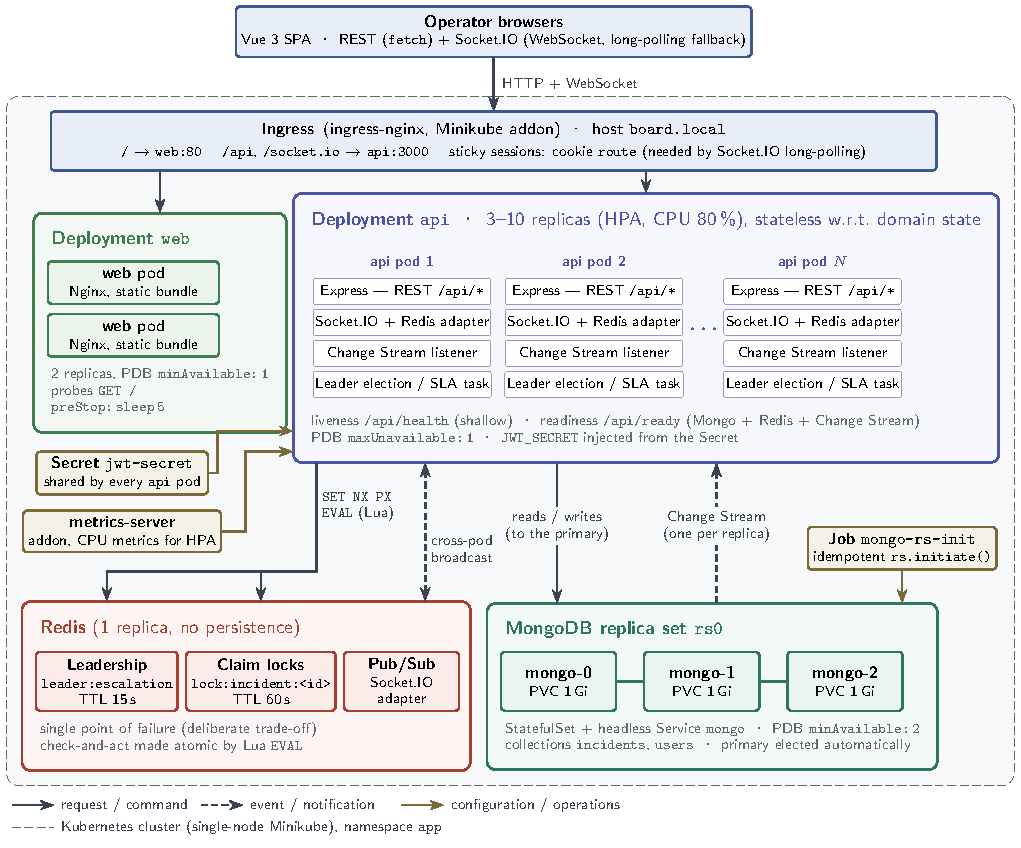
\includegraphics[width=\textwidth]{figures/architettura.pdf}
  \caption{System architecture: request routing through the Ingress, the \texttt{web} and \texttt{api} Deployments, and the shared Redis and MongoDB backing services. Solid arrows are requests and commands; dashed arrows are events: each \texttt{api} replica receives incident changes from its own Change Stream, while claim and presence events cross replicas through Redis Pub/Sub.}
  \label{fig:architecture}
\end{figure}

\paragraph{Network placement.} In the validated deployment, all components run within a single Kubernetes cluster (a single-node Minikube instance), but each is an independently scheduled Pod communicating exclusively over the cluster's internal network. The architecture therefore does not preclude spreading these components across multiple nodes in a production-grade cluster; this was intentionally left as a deployment-time concern rather than an application-level one. 
 
\paragraph{Component discovery.} Services are located through Kubernetes, with no custom mechanism in the application code:
%
\begin{itemize}
  \item \texttt{api}, \texttt{web} and \texttt{redis} are reached through \texttt{ClusterIP} Services and the cluster DNS (e.g., \texttt{redis.app.svc.cluster.local}). The Ingress, instead, forwards external traffic directly to the pods listed as the Service's endpoints, which is what allows its affinity cookie to pin a client to one \texttt{api} pod.
  \item MongoDB uses a \emph{headless} Service with the StatefulSet's stable per-pod names (\texttt{mongo-0.mongo}, \ldots), because replica-set members must be reachable individually rather than load-balanced.
  \item Externally, the Ingress exposes a single hostname (\texttt{board.local}) with path-based routing.
\end{itemize}
%
Beyond this, the MongoDB driver discovers the current primary by itself from the seed list in \texttt{MONGO\_URL}, and the \texttt{api} replicas never address each other: they meet only through Redis (adapter channels, \texttt{io.fetchSockets()}, the \texttt{leader:escalation} key), so the HPA can add or remove replicas without reconfiguring the others.
 
\subsection{Modelling}\label{modelling}
 
\paragraph{Domain entities.} The core entity is the \textbf{Incident} (\texttt{title}, \texttt{status} $\in \{\texttt{open}, \texttt{escalated}, \texttt{closed}\}$, \texttt{createdBy}, \texttt{closedBy}, \texttt{version}, \texttt{updatedAt}). Two further concepts are kept outside it. The \textbf{Operator} has persistent credentials (username and bcrypt hash), but its \emph{presence} exists only while its WebSocket connection is open. The \textbf{Claim}, the exclusive right to work on an incident, is never written to MongoDB: it is a Redis key with a time-to-live, which is nevertheless read back into the board snapshot at every hydration (\cref{database-querying}). \Cref{fig:class-diagram} shows these entities together with the backend modules that operate on them.

\begin{figure}[htbp]
  \centering
  % Sorgente TikZ in figures/diagramma-classi.tex: va ricompilato a parte dopo ogni modifica.
  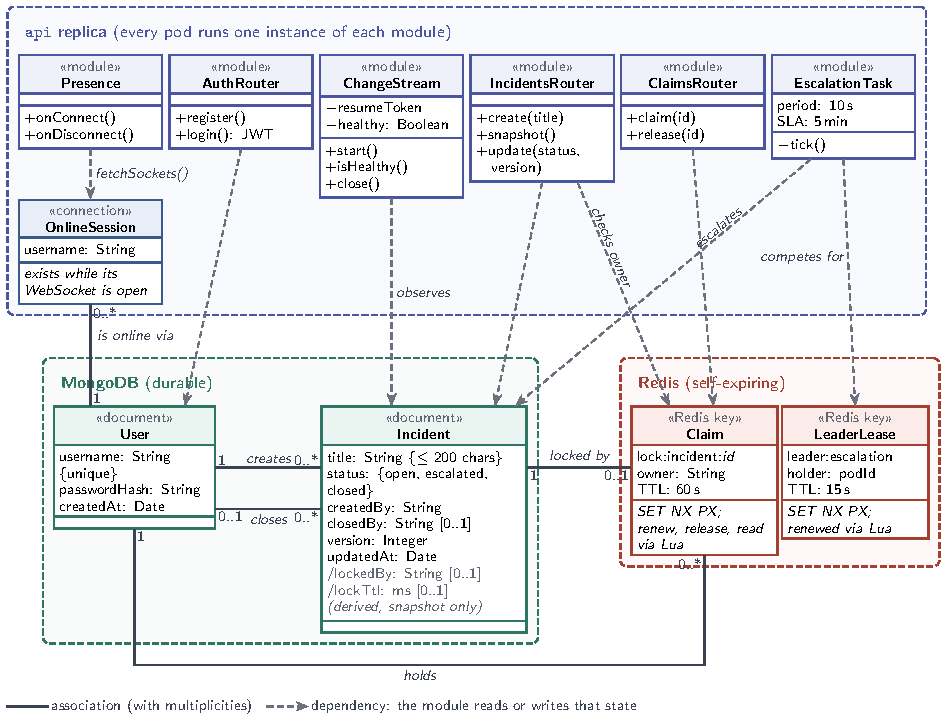
\includegraphics[width=\textwidth]{figures/diagramma-classi.pdf}
  \caption{Class diagram.}
  \label{fig:class-diagram}
\end{figure}
 
\paragraph{Mapping to infrastructure.} This distinction directly reflects each entity's durability requirement:
%
\begin{itemize}
  \item The \textbf{Incident} must survive pod restarts, rolling updates, and node failures, and is therefore stored in MongoDB, replicated across the 3-node Replica Set.
  \item The \textbf{Claim} and the \textbf{leadership mandate} are, by design, short-lived and self-expiring; persisting them durably would be both unnecessary and actively harmful (a durable lock that outlives its holder's crashed connection would deadlock the resource). They are therefore stored in Redis, an in-memory store with native TTL support.
  \item The \textbf{Operator}'s \emph{credentials} are persisted in MongoDB, because authentication must outlive any single connection or pod; the operator's \emph{presence}, by contrast, is not persisted anywhere: it exists only as \texttt{socket.data.username} on a live connection, discoverable cluster-wide on demand via \texttt{io.fetchSockets()}, and simply ceases to exist the moment the connection closes.
\end{itemize}
 
\paragraph{Domain events.} \texttt{IncidentCreated}, \texttt{IncidentClaimed}, \texttt{IncidentReleased}, \texttt{IncidentResolved}, \texttt{IncidentEscalated}, and \texttt{PresenceChanged} are the events that drive the system. They are realized, respectively, as: MongoDB Change Stream notifications for the events that mutate the Incident's persistent state (created, resolved, escalated), and direct Socket.IO broadcasts for the events that mutate only ephemeral Redis state (claimed, released, presence changed).
 
\paragraph{Messages.} Two distinct message categories are exchanged: 
\begin{itemize}
  \item \textbf{commands} (client $\to$ server, over REST: \texttt{POST /incidents}, \texttt{POST}/\texttt{DELETE .../claim}, \texttt{PATCH /incidents/:id}), which expect a definite success/failure reply and change system state.
  \item \textbf{events} (server $\to$ client, over Socket.IO: \texttt{incident\_update}, \texttt{incident\_locked}/\texttt{incident\_unlocked}, \texttt{users\_update}, \texttt{resync\_required}), which are fire-and-forget notifications with no expected reply. There are no \emph{queries} beyond \texttt{GET /api/incidents}, used to hydrate a client's local state at connection time, after every reconnect, and whenever the server itself asks for a resynchronization via \texttt{resync\_required} (\cref{fault-tolerance}) --- after hydration, the client never polls again, relying entirely on the event stream to stay current.
\end{itemize}
 
\paragraph{System state.} The authoritative state of the system is split across two stores by design: MongoDB holds the durable Incident collection; Redis holds transient coordination state (locks, leadership). Each connected client additionally holds a \emph{derived}, client-local copy of a filtered view of that state (the \texttt{incidents} and \texttt{onlineUsers} reactive references in the Vue application), which is not authoritative and is kept eventually consistent with the server through the event stream and the reconnect-time resynchronization.
 
\subsection{Interaction}\label{interaction}
 
Two interaction patterns coexist, cleanly separated by direction:
%
\begin{itemize}
  \item \textbf{Client $\to$ server: request/response.} Every mutation (create, claim, release, resolve) is a synchronous HTTP call that yields a definite outcome (\texttt{2xx} success or \texttt{4xx}/\texttt{5xx} failure) before the client considers the action complete.
  \item \textbf{Server $\to$ client: publish/subscribe.} All state changes are broadcast to every interested client without any client explicitly requesting them, and without the server tracking who has or hasn't yet seen a given update. No server-initiated request ever targets one specific client.
\end{itemize}
 
Within the publish/subscribe direction, two further sub-patterns are used depending on the origin of the change, both of which were the subject of extensive tuning during development:
%
\begin{itemize}
  \item Changes to \textbf{persistent} state (create, resolve, escalate) are captured by MongoDB Change Streams and broadcast via \texttt{io.local.emit()} because every \texttt{api} pod independently watches the same Change Stream and would otherwise re-broadcast an event that every other pod has \emph{already} independently received and forwarded to its own clients, causing duplicate delivery.
  \item Changes to \textbf{ephemeral} state not reflected in MongoDB (claim, release, presence) are broadcast via \texttt{io.emit()}, which \emph{does} need to cross pod boundaries through the Redis adapter, since only one pod knows the change happened: the one that served the claim or release request, or the one where an operator's WebSocket connected or disconnected. Resolving an incident uses both channels at once: the status change reaches clients through the Change Stream, while the release of its lock is announced with \texttt{io.emit()}.
\end{itemize}
%
A third case has no originating pod at all: when a claim lock simply \emph{expires} in Redis, no request was served and no pod is aware that anything happened, so no event can be emitted. This category of change is therefore not propagated by a broadcast but \emph{predicted} by each client independently, from the remaining time-to-live the server sends alongside every lock. Overlooking this third case was the root of a defect described in \cref{ds-features}, \emph{Evolvability, Maintainability}.

\paragraph{Sequence diagrams.} The four most significant interactions are shown below, each with two \texttt{api} pods so that it is visible which messages cross pod boundaries. \Cref{fig:seq-login} covers login, the WebSocket handshake, presence and the hydration of the board. \Cref{fig:seq-claim} shows a claim with its three possible outcomes. \Cref{fig:seq-resolve} shows a resolution, where the two channels run in parallel: the release of the lock travels through Redis Pub/Sub, the status change through the Change Stream of every pod. \Cref{fig:seq-escalation} shows the SLA escalation run by the leader, which writes to MongoDB and leaves the notification to the Change Streams.

\begin{figure}[htbp]
  \centering
  % Sorgente TikZ in figures/diagrammi-sequenza.tex (una pagina per diagramma): va ricompilato a parte dopo ogni modifica.
  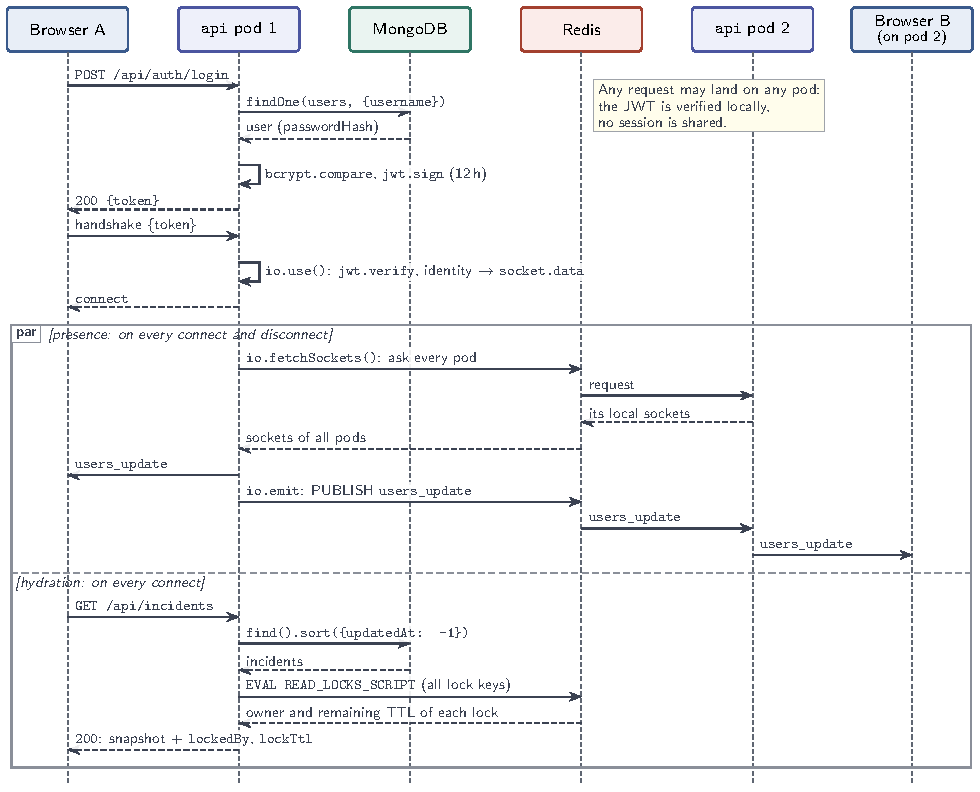
\includegraphics[width=\textwidth,page=1]{figures/diagrammi-sequenza.pdf}
  \caption{Login, WebSocket handshake, presence and hydration. Presence and hydration both start at every connection and run concurrently.}
  \label{fig:seq-login}
\end{figure}

\begin{figure}[htbp]
  \centering
  % Sorgente TikZ in figures/diagrammi-sequenza.tex (una pagina per diagramma): va ricompilato a parte dopo ogni modifica.
  \includegraphics[width=\textwidth,page=2]{figures/diagrammi-sequenza.pdf}
  \caption{Claiming an incident. The claim is idempotent for the operator who already holds the lock; the \texttt{409} is reserved for a conflict with another operator.}
  \label{fig:seq-claim}
\end{figure}

\begin{figure}[htbp]
  \centering
  % Sorgente TikZ in figures/diagrammi-sequenza.tex (una pagina per diagramma): va ricompilato a parte dopo ogni modifica.
  \includegraphics[width=\textwidth,page=3]{figures/diagrammi-sequenza.pdf}
  \caption{Resolving an incident. The \texttt{PATCH} requires owning the lock, and the update is conditioned on both the version and the allowed source status.}
  \label{fig:seq-resolve}
\end{figure}

\begin{figure}[htbp]
  \centering
  % Sorgente TikZ in figures/diagrammi-sequenza.tex (una pagina per diagramma): va ricompilato a parte dopo ogni modifica.
  \includegraphics[width=\textwidth,page=4]{figures/diagrammi-sequenza.pdf}
  \caption{SLA escalation. Every pod competes for the lease at every tick; only the leader writes, and every pod notifies its own clients from its Change Stream.}
  \label{fig:seq-escalation}
\end{figure}


\subsection{Behaviour}\label{behaviour}
 
\begin{itemize}
  \item \textbf{\texttt{api} pods} are stateless with respect to domain data: nothing about an incident, a claim, or a user is cached in a pod's own memory across requests. Each pod reacts to three independent stimuli: (1) incoming REST requests, handled synchronously; (2) events pushed by its own MongoDB Change Stream subscription, handled asynchronously and forwarded only to its own locally-connected sockets; (3) an internal timer (every 10 seconds) that drives both the leader-election attempt and, if leadership is held, the escalation scan --- this third stimulus is self-generated, not triggered by any external message.
  \item \textbf{MongoDB} accepts writes only on the elected primary, which replicates them to the two secondaries via the oplog; if the primary becomes unreachable, the remaining nodes run an automatic election (majority-based) to promote a new primary, with no application-level intervention required.
  \item \textbf{Redis} is purely reactive and carries no domain logic of its own: it only executes the commands (\texttt{SET NX PX}, \texttt{EVAL} of the Lua scripts, \texttt{GET}, \texttt{DEL}) issued by the \texttt{api} pods, and expires keys autonomously once their TTL elapses.
  \item \textbf{The Vue.js client} does not update its local state optimistically on user action; it waits for the server's response (for the direct outcome of its own command) and for the corresponding broadcast event (for the canonical, server-confirmed state), which keeps the client's view a strict function of what the server has actually confirmed, rather than a prediction that could be wrong and require a visible correction later. 
\end{itemize}
 
\paragraph{State diagrams.} Four components have an explicit lifecycle worth modelling. An \textbf{incident} (\cref{fig:state-incident}) combines its durable status in MongoDB with the ephemeral claim in Redis: the two dimensions are independent, which is why an incident can be escalated while someone is working on it. Each \texttt{api} pod has two internal state machines: its \textbf{Change Stream} (\cref{fig:state-changestream}), which decides whether the pod is ready to receive traffic, and its role in the \textbf{leader election} (\cref{fig:state-leader}). Finally, each \textbf{client session} (\cref{fig:state-client}) moves between connecting, hydrating from the REST snapshot and following live events.

\begin{figure}[htbp]
  \centering
  % Sorgente TikZ in figures/diagrammi-stato.tex (una pagina per diagramma): va ricompilato a parte dopo ogni modifica.
  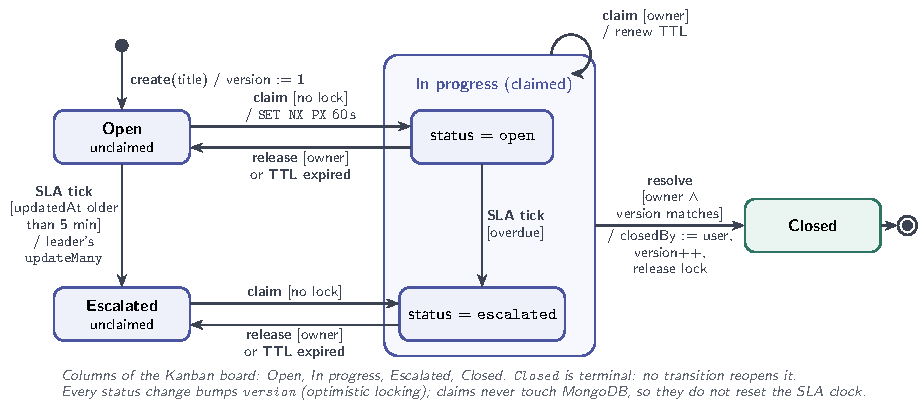
\includegraphics[width=\textwidth,page=1]{figures/diagrammi-stato.pdf}
  \caption{Incident lifecycle. The \emph{In progress} composite state corresponds to the claimed incidents; its two substates keep the status that the incident returns to when the claim is released or expires.}
  \label{fig:state-incident}
\end{figure}

\begin{figure}[htbp]
  \centering
  % Sorgente TikZ in figures/diagrammi-stato.tex (una pagina per diagramma): va ricompilato a parte dopo ogni modifica.
  \includegraphics[width=\textwidth,page=2]{figures/diagrammi-stato.pdf}
  \caption{Change Stream of a single \texttt{api} pod. Only the \emph{Streaming} state passes the readiness probe; the retry reschedules itself even when \texttt{watch()} fails synchronously.}
  \label{fig:state-changestream}
\end{figure}

\begin{figure}[htbp]
  \centering
  % Sorgente TikZ in figures/diagrammi-stato.tex (una pagina per diagramma): va ricompilato a parte dopo ogni modifica.
  \includegraphics[width=\textwidth,page=3]{figures/diagrammi-stato.pdf}
  \caption{Leader election, as seen by a single \texttt{api} pod at every 10-second tick.}
  \label{fig:state-leader}
\end{figure}

\begin{figure}[htbp]
  \centering
  % Sorgente TikZ in figures/diagrammi-stato.tex (una pagina per diagramma): va ricompilato a parte dopo ogni modifica.
  \includegraphics[width=\textwidth,page=4]{figures/diagrammi-stato.pdf}
  \caption{Client session in the browser. The \emph{generation} counter discards snapshots that arrive after a newer resynchronization has started.}
  \label{fig:state-client}
\end{figure}

 
\subsection{Data and Consistency Issues}\label{data-and-consistency-issues}
 
\paragraph{What is stored, and where.} Incidents are the only data that must persist beyond a single request or connection; they are stored in \textbf{MongoDB} as documents. The document model was chosen because incidents are naturally semi-structured records whose schema evolved incrementally over the project's development (e.g., the \texttt{escalated} status and the \texttt{closedBy} field were both introduced after the initial design) without requiring a formal migration step. Coordination data (locks, leadership) is stored in \textbf{Redis} as plain key-value pairs, chosen because the access pattern is a pure read/write/expire on independent keys with no relational structure, and because lock contention needs sub-millisecond latency that an in-memory store provides naturally.
 
\paragraph{Query and write patterns.} \texttt{api} pods are the only components that ever query or write MongoDB and Redis; the client never talks to either data store directly, always mediating through the REST/Socket.IO layer. Concurrent \emph{reads} are unrestricted and require no coordination (both MongoDB and Redis handle concurrent reads natively). Concurrent \emph{writes} are expected and must be explicitly coordinated: this is precisely the motivation behind the two concurrency-control mechanisms of \cref{non-functional-requirements} --- optimistic locking detects conflicting concurrent writes to the \emph{same} Incident document, and the distributed lock prevents two operators from concurrently claiming the same Incident in the first place.
 
\paragraph{Shared data.} The Incidents collection is, by design, shared read/write state across every \texttt{api} replica --- this sharing is the entire point of keeping the application tier stateless and horizontally scalable. The same is true of the Redis keyspace: coordination only works if every replica observes the same lock and leadership state, which is why a single shared Redis instance (rather than one per pod) is a hard requirement, not an implementation convenience.
 
\paragraph{Consistency model.} The system provides \textbf{strong consistency} for writes to the primary (a successful write is immediately visible to any subsequent read against the primary) and \textbf{eventual consistency} for propagation to connected clients: a change is always durably committed to MongoDB \emph{before} any client is notified of it, but different clients may observe the notification at slightly different times depending on Change-Stream and network latency. This asymmetry is a deliberate, accepted trade-off: the domain (a SOC dashboard) tolerates sub-second staleness in what operators \emph{see}, but never tolerates staleness or loss in what is actually \emph{recorded} as the incident's state.
 
\subsection{Fault-Tolerance}\label{fault-tolerance}
 
\paragraph{Replication.} MongoDB runs as a 3-node Replica Set, which survives the loss of one node without losing data or write availability. Redis is deliberately \emph{not} replicated (\cref{ds-features}, \emph{Fault Tolerance, Dependability}): it holds coordination state, not the system of record, so its failure costs availability while it is down and the active claims, which no one reconstructs, but never durable data; the leadership is simply re-elected at the next tick. The 3--10 \texttt{api} pods are interchangeable stateless workers rather than replicas of any data.
 
\paragraph{Heartbeats, timeouts, and retries.}
%
\begin{itemize}
  \item \textbf{Probes.} The liveness probe (\texttt{/api/health}) is shallow and the readiness probe (\texttt{/api/ready}) is deep: it checks MongoDB, Redis and the pod's own Change Stream. A failing dependency therefore takes a pod out of the Service without restarting it.
  \item \textbf{Leases.} Claims and leadership are Redis keys with a TTL: a crashed holder needs no failure detector, because its lock simply expires.
  \item \textbf{Connection heartbeat.} Socket.IO's ping/pong detects dead connections, which keeps the presence list computed with \texttt{io.fetchSockets()} correct.
  \item \textbf{Client retries.} The Socket.IO client reconnects automatically, and the resynchronization-generation counter (NFR7) discards out-of-date snapshots.
  \item \textbf{Change Stream recovery.} A broken stream is rebuilt with exponential backoff (1\,s doubling up to 30\,s) and \texttt{resumeAfter}, so the changes made during the outage are replayed. If the resume token is no longer in the oplog, the stream restarts from the present and the pod sends \texttt{resync\_required} to its clients. If the stream is still down after 20\,s, the pod disconnects its clients so that they reconnect to a healthy pod.
\end{itemize}
 
\paragraph{Error handling.} Every REST handler catches its errors and answers with a specific status (\texttt{400}/\texttt{404} for invalid input, \texttt{409} for a lock or version conflict, \texttt{500} otherwise) instead of crashing the process. A failure to reach MongoDB or Redis \emph{at startup}, instead, is fatal by design (\texttt{process.exit(1)}): Kubernetes restarts the pod rather than letting it serve traffic half-initialized. On the frontend, every action checks the response status and shows a notification on failure, including network errors and response bodies that are not valid JSON.
 
\subsection{Availability}\label{availability}
 
\paragraph{Caching.} No read cache is used for Incident data: every \texttt{GET} reads MongoDB directly. This is a deliberate simplicity choice --- the read volume expected from a SOC dashboard with a handful of concurrent operators does not justify the added complexity of cache invalidation. Redis, despite superficially resembling a cache, is never used to cache MongoDB reads in this system; its only roles are coordination (locks, leadership) and message brokering (the Socket.IO adapter).
 
\paragraph{Load balancing.} The Ingress load-balances HTTP and WebSocket traffic across the $\geq 3$ \texttt{api} replicas, using cookie-based \textbf{sticky sessions} specifically because Socket.IO's HTTP long-polling fallback transport requires successive requests within one handshake to reach the \emph{same} backend process; a plain stateless REST call would not need this affinity, but the shared Ingress rule applies it uniformly for simplicity. This mechanism works together with the \texttt{HorizontalPodAutoscaler}, which keeps the pool of backends elastic under load (\cref{non-functional-requirements}).
 
\paragraph{Behaviour under network partitioning.} Several partition scenarios are explicitly handled, each favouring a different side of the CAP trade-off depending on what is partitioned:
%
\begin{itemize}
  \item If an \texttt{api} pod loses connectivity to Redis or MongoDB, or its Change Stream dies without being immediately re-establishable, \texttt{/api/ready} starts failing and Kubernetes removes the pod from the Service's endpoint list --- it stops receiving traffic but is \emph{not} killed, and rejoins automatically once connectivity is restored. This favours \textbf{consistency and correctness} (no pod serves requests it cannot fulfil correctly) over that individual pod's availability.
  \item If a MongoDB secondary is partitioned from the primary, it simply falls behind and resynchronizes once the partition heals, without disrupting the primary's availability.
  \item If the primary itself is partitioned from the majority of the Replica Set, it steps down to avoid a split-brain scenario (two nodes both believing they are primary), again favouring \textbf{consistency (CP)} over the availability of the minority side --- the design explicitly accepts that the minority partition becomes unavailable for writes rather than risk divergent, unreconcilable incident data.
\end{itemize}
 
\subsection{Security}\label{security}
 
\paragraph{Authentication.} Operators register with a username and a password of at least 8 characters; the password is stored only as a bcrypt hash, and the uniqueness of the username is enforced by a unique index rather than by an application-level check, which would race across replicas. Login answers with the same error for an unknown user and a wrong password, so it does not reveal which usernames exist, and issues a JWT (subject: the username, validity: 12 hours) signed with a secret shared by every \texttt{api} replica through a Kubernetes \texttt{Secret}. The token is required on every REST call (\texttt{Authorization: Bearer}) and on the Socket.IO handshake, and any pod can verify it locally: no session state is kept on the server. The browser keeps it in \texttt{sessionStorage}, so it survives a page reload but not the closing of the tab. The known limits are deliberate simplifications (\cref{ds-features}, \emph{Security, Trust}): authentication is single-factor, there is no password reset, account lockout or rate limiting on login, and the WebSocket token is checked only at the handshake, so an open connection outlives the expiry of its token.

\paragraph{Authorization.} There is a single role: every authenticated operator can create incidents and claim any unclaimed one. Releasing and resolving, instead, require \emph{owning} the incident's Redis lock: the server answers \texttt{409} both when the lock belongs to someone else and when there is no lock at all, so the mutual exclusion cannot be bypassed by simply not claiming (NFR2). The lock therefore acts as a capability for a single incident, and it is anchored to a verified identity: its value, like \texttt{createdBy} and \texttt{closedBy}, is always the username taken from the caller's JWT and never from the request body.

\paragraph{Input validation.} Every route validates its input before touching the stores: incident titles must be non-empty and at most 200 characters, a status must belong to the allowed set and follow an allowed transition (a closed incident cannot be reopened), and the optimistic-locking \texttt{version} is mandatory. Incident identifiers are checked for format and existence before being turned into a Redis key, which prevents a client from creating arbitrary keys or announcing a lock on an incident that does not exist.

\paragraph{Cryptography and secrets.} Cryptography is used only for authentication: bcrypt for passwords and HMAC-signed JWTs for tokens. Nothing travels encrypted: the Ingress serves plain HTTP, so passwords and tokens cross the network in clear, and the traffic between the \texttt{api} pods and MongoDB or Redis is unencrypted as well; neither store requires authentication, and no data is encrypted at rest. Moreover, the \texttt{Secret} committed in the repository holds a placeholder value meant for the local demo, which a real deployment must generate outside the repository. Transport and at-rest encryption are listed among the future works (\cref{future-works}).
 
\section{Implementation}\label{implementation}

\subsection{Technology Stack}\label{tech-stack}

\begin{itemize}
  \item \textbf{Frontend:} a single-page application in Vue~3 (Composition API, \texttt{<script setup>}), built with Vite. \texttt{socket.io-client} keeps the real-time channel, Chart.js (through \texttt{vue-chartjs}) draws the dashboard chart, and \texttt{vue-toastification} shows the notifications.
  \item \textbf{Backend:} Node.js~20 with Express~5 for the REST API and Socket.IO~4 for the WebSocket server, extended across pods by \texttt{@socket.io/redis-adapter}. Authentication uses \texttt{jsonwebtoken} and \texttt{bcryptjs}; the stores are reached through the official \texttt{mongodb} and \texttt{redis} (node-redis) drivers.
  \item \textbf{Database:} MongoDB~6 as a 3-member replica set, the durable store of incidents and users and the source of the Change Streams; Redis~7 as a single in-memory instance for the claim locks, the leader lease and the Socket.IO Pub/Sub.
  \item \textbf{Distributed infrastructure:} Kubernetes, validated on Minikube: Deployments for \texttt{api}, \texttt{web} and Redis, a StatefulSet with a headless Service for MongoDB, a one-shot Job for the replica-set initialization, an ingress-nginx Ingress with cookie affinity, a HorizontalPodAutoscaler fed by \texttt{metrics-server}, PodDisruptionBudgets and a Secret for the JWT key.
  \item \textbf{Containerisation:} Docker. The \texttt{api} image is based on \texttt{node:20-alpine} with production dependencies only; the \texttt{web} image is a multi-stage build that compiles the bundle on \texttt{node:20-alpine} and serves it with \texttt{nginx:alpine}. MongoDB and Redis use the official \texttt{mongo:6} and \texttt{redis:7} images.
  \item \textbf{API:} REST over HTTP with JSON bodies under \texttt{/api} (authentication, incidents, claims, health probes), authenticated with a \texttt{Bearer} JWT; server-to-client events over Socket.IO, on WebSocket with a long-polling fallback.
\end{itemize}

\subsection{Network Protocols}\label{network-protocols}

Two application-level protocols coexist, each chosen for a specific interaction pattern:

\paragraph{HTTP/1.1 over TCP} is used for all \textbf{command} (mutation) interactions from the client to the server. The REST API exposed by Express.js defines five endpoints:
%
\begin{itemize}
  \item \texttt{POST /api/incidents} --- create a new incident;
  \item \texttt{GET /api/incidents} --- retrieve the full incident list, each document enriched with the current holder of its claim and that claim's remaining time-to-live (used at connect time, on every reconnect, and on server-requested resynchronization);
  \item \texttt{POST /api/incidents/:id/claim} --- acquire the distributed lock on an incident;
  \item \texttt{DELETE /api/incidents/:id/claim} --- explicitly release a held lock;
  \item \texttt{PATCH /api/incidents/:id} --- resolve an incident (with optimistic-locking version check and server-side lock verification).
\end{itemize}
%
HTTP was chosen because every mutation requires an unambiguous, synchronous success-or-failure response (e.g., ``did I get the lock or not?''), which request/response semantics provide naturally. 

\paragraph{WebSocket (via Socket.IO)} is used for all \textbf{event} (notification) interactions from the server to connected clients. The Socket.IO library negotiates a WebSocket upgrade after an initial HTTP handshake, falling back to HTTP long-polling if WebSocket is unavailable. The server emits five event types:
%
\begin{itemize}
  \item \texttt{incident\_update} --- carries a MongoDB Change Stream document (insert or update) describing a persistent state change;
  \item \texttt{incident\_locked} / \texttt{incident\_unlocked} --- notifies all clients of ephemeral lock state changes; \texttt{incident\_locked} also carries the claim's time-to-live, so that each client can expire the lock locally when no event will announce its natural expiry;
  \item \texttt{users\_update} --- broadcasts the current list of connected operators;
  \item \texttt{resync\_required} --- asks the pod's own clients to re-hydrate from \texttt{GET /api/incidents}, emitted when the pod knows it has lost a segment of the change feed and cannot replay it (\cref{fault-tolerance}).
\end{itemize}
%
WebSocket was chosen over polling because the design requires near-real-time propagation of every state change to every connected client.

\paragraph{Redis protocol (RESP).} The \texttt{api} pods communicate with Redis using the native Redis Serialization Protocol over TCP, mediated by the \texttt{redis} npm package (v6). This includes standard commands (\texttt{SET}, \texttt{GET}, \texttt{DEL}, \texttt{PING}) and Lua script evaluation (\texttt{EVAL}) for atomic lock operations.

\paragraph{MongoDB Wire Protocol.} The \texttt{api} pods communicate with the MongoDB Replica Set using the MongoDB binary wire protocol over TCP, mediated by the official \texttt{mongodb} npm driver (v7). The connection string enumerates all three replica-set members (\texttt{mongo-0.mongo:27017}, \texttt{mongo-1.mongo:27017}, \texttt{mongo-2.mongo:27017}) with \texttt{replicaSet=rs0}, enabling automatic primary discovery and failover-transparent reconnection.

\subsection{In-Transit Data Representation}\label{data-representation}

\textbf{JSON} is used as the sole serialization format for all inter-component communication that crosses a network boundary in the application layer:
%
\begin{itemize}
  \item \textbf{REST API:} both request bodies (e.g., \texttt{\{"title": "...", "status": "open", "createdBy": "alice"\}}) and response bodies are JSON. The Express.js middleware \texttt{express.json()} parses incoming bodies, and every route handler returns a JSON object via \texttt{res.json()}.
  \item \textbf{Socket.IO events:} each emitted event carries a JSON payload. For \texttt{incident\_update}, the payload is the raw MongoDB Change Stream document (which is already a JSON-like BSON structure, automatically serialized to JSON by the driver). For \texttt{incident\_locked} the payload is \texttt{\{id, lockedBy, ttl\}} and for \texttt{incident\_unlocked} simply \texttt{\{id\}}; for presence, a plain array of username strings; \texttt{resync\_required} carries no payload at all, being a pure signal. The \texttt{ttl} field is deliberately a \emph{relative} duration in milliseconds rather than an absolute expiry timestamp: an absolute deadline would only be interpretable by a client whose clock agrees with the cluster's, and a few seconds of skew would make locks expire visibly too early or too late.
  \item \textbf{MongoDB $\leftrightarrow$ driver:} the driver uses BSON (Binary JSON) on the wire, which is transparently serialized/deserialized by the \texttt{mongodb} npm package; the application code only ever manipulates plain JavaScript objects.
  \item \textbf{Redis $\leftrightarrow$ driver:} Redis values are plain UTF-8 strings (usernames, pod identifiers); no structured serialization is needed because each key holds a single scalar value.
\end{itemize}
%
\subsection{Database Querying}\label{database-querying}

MongoDB is queried through the fluent API of the official Node.js driver.

\paragraph{Writes.}
%
\begin{itemize}
  \item \texttt{insertOne} creates an incident with \texttt{status: 'open'}, \texttt{version: 1} and \texttt{updatedAt}, and registers a user; the uniqueness of usernames is enforced by a unique index.
  \item \texttt{updateOne(\{\_id, version, status: \{\$in: allowed sources\}\}, \{\$set: ..., \$inc: \{version: 1\}\})} implements optimistic locking: the update applies only if nobody has changed the document since the client read it and the transition is allowed from its current status.
  \item \texttt{updateMany(\{status: 'open', updatedAt: \{\$lt: threshold\}\}, ...)} escalates every overdue incident in a single round-trip.
\end{itemize}

\paragraph{Reads.} The board snapshot is \texttt{find(\{\}).sort(\{updatedAt: -1\})}, enriched with the holder and remaining TTL of each claim read from Redis, so that every client hydrates to the same state whenever it connects; documents are read before locks, so a lock acquired in between is reported rather than lost. The other reads are point lookups: the user at login, the existence of an incident before any claim, and its current status and version after a failed update, to tell a version conflict from a forbidden transition.

\paragraph{Change Streams.} \texttt{watch([], \{fullDocument: 'updateLookup'\})} streams every insert and update with the full document, replacing any polling. Each event's \texttt{\_id} is kept as a resume token and passed as \texttt{resumeAfter} when the cursor is rebuilt; the driver already retries resumable errors such as a primary failover, so the application only handles the rest (\cref{fault-tolerance}).

\paragraph{Redis.} Single-key commands (\texttt{SET NX PX}, \texttt{GET}) plus three Lua scripts, which Redis executes atomically:
%
\begin{itemize}
  \item \texttt{RENEW\_LOCK\_SCRIPT} extends a key's TTL only if it still belongs to the caller; it renews both the leadership and the claim of its current holder.
  \item \texttt{RELEASE\_LOCK\_SCRIPT} deletes a claim only if it still belongs to the caller, so an expired lock taken over by someone else is never deleted by mistake.
  \item \texttt{READ\_LOCKS\_SCRIPT} returns owner and remaining TTL of every existing lock in one call: the two values refer to the same instant, and hydration costs one round-trip regardless of the size of the board.
\end{itemize}

\subsection{Technological Details}\label{technological-details}

\subsubsection{Backend Runtime and Frameworks}

\begin{itemize}
  \item \textbf{Node.js~20} (Alpine-based Docker image, \texttt{node:20-alpine}): chosen as the application runtime because its single-threaded, event-loop-based execution model is well suited to hosting both synchronous request handlers and long-lived WebSocket connections in the same process, without the thread-management overhead of a multi-threaded server.
  \item \textbf{Express.js~5}: provides the HTTP routing layer. An \texttt{express.Router()} instance mounts all endpoints under the \texttt{/api} prefix; the \texttt{express.json()} middleware handles request body parsing; and \texttt{cors()} is configured with the \texttt{CORS\_ORIGIN} environment variable to restrict cross-origin requests in deployment.
  \item \textbf{Socket.IO~4}: provides the WebSocket transport layer, with automatic fallback to HTTP long-polling if WebSocket upgrade fails. The \texttt{@socket.io/redis-adapter} (v8) bridges all Socket.IO instances across the \texttt{api} pods so that events emitted with \texttt{io.emit()} are propagated cluster-wide via Redis Pub/Sub.
  \item \textbf{mongodb~7} (official Node.js driver): provides the connection to the MongoDB Replica Set, including Change Streams support and automatic primary failover handling.
  \item \textbf{redis~6} (Node.js client): provides the connection to Redis for distributed locks, leader election, and the Socket.IO adapter's Pub/Sub channels. Two client instances are created (\texttt{pubClient} and \texttt{subClient}), as required by the Redis adapter which needs dedicated publish and subscribe connections.
\end{itemize}

\subsubsection{Frontend Framework and Libraries}

\begin{itemize}
  \item \textbf{Vue.js~3} with the Composition API (\texttt{<script setup>}): the SPA framework. The entire dashboard is a single \texttt{App.vue} component using Vue's reactivity system (\texttt{ref}, \texttt{computed}) to derive filtered views of the incident list and KPI counters from a single reactive \texttt{incidents} array that is kept current by the Socket.IO event stream.
  \item \textbf{Vite~8}: the build tool and development server. The production build (triggered by \texttt{npm run build} inside the multi-stage Dockerfile) produces a static bundle served by Nginx.
  \item \textbf{socket.io-client~4}: the browser-side Socket.IO library. The connection is established with \texttt{io('/', \{path: '/socket.io', auth: \{token\}\})}, which leverages the Ingress's path-based routing to reach the \texttt{api} service; the token is the same JWT used for REST calls, verified by the server on the handshake.
  \item \textbf{vue-toastification~2}: provides non-blocking toast notifications for all real-time events (new tickets, escalations, resolutions by others) and for local operation failures (claim conflicts, version conflicts, network errors). Configured in \texttt{main.js} with bottom-right positioning, 5-second timeout, and a progress bar.
  \item \textbf{Chart.js~4} (via \texttt{vue-chartjs~5}): renders the bar chart in the ``Incidents Status Overview'' card, with reactive data bindings to the computed KPI properties so the chart updates automatically as the incident counts change.
\end{itemize}

\subsubsection{Containerization}

Both application components use \textbf{Docker} multi-stage or single-stage builds:
%
\begin{itemize}
  \item \textbf{API image:} a single-stage build from \texttt{node:20-alpine}. The \texttt{Dockerfile} copies \texttt{package*.json} first and runs \texttt{npm ci --only=production} to leverage Docker's layer cache, then copies the application code. The entrypoint is \texttt{node index.js}.
  \item \textbf{Web image:} a multi-stage build. Stage~1 (\texttt{node:20-alpine}) installs dependencies and runs \texttt{npm run build} to compile the Vue SPA into static assets. Stage~2 copies the \texttt{dist/} output into an \texttt{nginx:alpine} image, producing a minimal container that serves only static files on port~80.
  \item \textbf{MongoDB and Redis:} use the official upstream images (\texttt{mongo:6} and \texttt{redis:7}) without custom Dockerfiles.
\end{itemize}
%
Both custom images set \texttt{imagePullPolicy: Never} in their Kubernetes manifests, instructing Kubernetes to use the locally-built images available in Minikube's Docker daemon rather than attempting to pull them from a remote registry.

\subsubsection{Orchestration (Kubernetes)}

The Kubernetes manifests in \texttt{k8s/} define the following resources, all deployed in the \texttt{app} namespace:
%
\begin{itemize}
  \item \textbf{API Deployment + Service} (\texttt{api.yaml}): a \texttt{Deployment} with 3 initial replicas, each running the \texttt{api:latest} image. Environment variables configure the MongoDB connection string (enumerating all three replica-set members), the Redis URL, and the CORS origin. The liveness probe (\texttt{/api/health}, shallow) and readiness probe (\texttt{/api/ready}, deep) are deliberately separated: a dependency outage only removes the pod from the Service's endpoint list (readiness failure) without restarting a healthy process (liveness would pass).

  \item \textbf{HorizontalPodAutoscaler} (\texttt{hpa.yaml}): targets the \texttt{api} Deployment, scaling between 3 and 10 replicas based on an 80\% average CPU utilization threshold.

  \item \textbf{MongoDB StatefulSet + Headless Service + ConfigMap + Job + PDB} (\texttt{mongo.yaml}): the most complex manifest, comprising five resources:
  %
  \begin{itemize}
    \item A \textbf{headless Service} (\texttt{clusterIP: None}) that provides stable per-pod DNS names (\texttt{mongo-0.mongo}, \texttt{mongo-1.mongo}, \texttt{mongo-2.mongo}), necessary because replica-set members must be individually addressable.
    \item A \textbf{ConfigMap} containing the \texttt{rs.initiate()} JavaScript invocation with the three member hostnames.
    \item A \textbf{StatefulSet} with 3 replicas, each running \texttt{mongo:6} with \texttt{--replSet rs0 --bind\_ip\_all}. Each pod has a \texttt{volumeClaimTemplate} requesting 1\,GiB of persistent storage, ensuring data survives pod restarts. Liveness and readiness probes execute \texttt{db.adminCommand('ping')} via \texttt{mongosh}.
    \item A one-shot \textbf{Job} (\texttt{mongo-rs-init}) that waits for all three members to be reachable, checks whether the replica set is already initialized, and if not, runs the \texttt{rs.initiate()} script and waits for a primary to be elected. The \texttt{backoffLimit: 5} and \texttt{restartPolicy: OnFailure} ensure the initialization is retried if it fails due to a transient readiness issue.
    \item A \textbf{PodDisruptionBudget} (\texttt{minAvailable: 2}) that prevents voluntary evictions (e.g., node drains, rolling updates) from disrupting more than one MongoDB pod at a time, preserving the quorum needed for automatic primary election.
  \end{itemize}

  \item \textbf{Redis Deployment + Service} (\texttt{redis.yaml}): a single-replica \texttt{Deployment} running \texttt{redis:7}, exposed via a \texttt{ClusterIP} Service on port~6379. No persistence, no replication --- a deliberate simplification documented in \cref{ds-features}.

  \item \textbf{Web Deployment + Service} (\texttt{web.yaml}): a single-replica \texttt{Deployment} running the Nginx-based \texttt{web:latest} image, exposed via a \texttt{ClusterIP} Service on port~80.

  \item \textbf{Ingress} (\texttt{ingress.yaml}): an Nginx Ingress resource configured for host \texttt{board.local} with three path-based routing rules:
  %
  \begin{itemize}
    \item \texttt{/} $\to$ \texttt{web:80} (static frontend assets);
    \item \texttt{/api} $\to$ \texttt{api:3000} (REST endpoints);
    \item \texttt{/socket.io} $\to$ \texttt{api:3000} (WebSocket transport).
  \end{itemize}
  %
  Cookie-based sticky sessions are enabled via annotations (\texttt{nginx.ingress.kubernetes.io/affinity: cookie}, cookie name \texttt{route}, 48-hour expiry) specifically because Socket.IO's HTTP long-polling fallback requires successive requests within the same handshake to reach the same backend pod.
\end{itemize}

\section{Validation}\label{validation}
\subsection{Acceptance Tests}\label{acceptance-test}

All validation was performed by \textbf{manual testing} on the live Minikube cluster, with several browser sessions and \texttt{curl}. Tests are grouped by mechanism rather than by requirement, and each lists the requirements it covers. Unless stated otherwise, the results were observed on the cluster; steps marked \emph{(expected)} cover behaviour introduced after the last validation round and describe what the code is meant to do, not an observed result.

Automating these scenarios would require orchestrating several browser sessions, injecting pod failures through the Kubernetes API, and waiting for infrastructure reactions such as probe recovery or HPA decisions. Playwright or Cypress could cover the browser side, but integrating them with \texttt{kubectl}-driven fault injection was beyond the time budget of a single-developer project.

In the commands below, \texttt{ALICE\_TOKEN} and \texttt{BOB\_TOKEN} are JWTs obtained from \texttt{POST /api/auth/login}. The identity behind every write (creator, lock owner, resolver) is always taken from the token, never from the request body.

\subsubsection{Real-Time Synchronization (FR2, FR3, NFR9)}

\begin{itemize}
  \item \textbf{Procedure:} log in as ``alice'' and ``bob'' in two browsers. As alice, create an incident, claim it and resolve it, observing bob's board after each step.
  \item \textbf{Expected:} the creation answers \texttt{201}, and every step appears on bob's board within about one second, with no refresh. At no point does the card appear in two columns at once, whichever of the lock-release and database events reaches the client first.
  \item \textbf{Result:} passed. Creation and resolution travel through the Change Stream (\texttt{incident\_update}, emitted by each pod to its own clients), the claim through the Redis adapter (\texttt{incident\_locked}). The columns are derived from both \texttt{status} and \texttt{lockedBy}, so any intermediate state falls into exactly one of them.
\end{itemize}

\subsubsection{Claim and Release (FR4, FR5)}

\begin{itemize}
  \item \textbf{Procedure:} claim the same incident concurrently as alice and bob:
  \begin{verbatim}
  curl -X POST http://board.local/api/incidents/<id>/claim \
       -H "Authorization: Bearer $ALICE_TOKEN" &
  curl -X POST http://board.local/api/incidents/<id>/claim \
       -H "Authorization: Bearer $BOB_TOKEN" &
  wait
  \end{verbatim}
  Then release the claim as its winner (\texttt{DELETE /api/incidents/<id>/claim}) and claim it again as the loser.
  \item \textbf{Expected:} exactly one claim answers \texttt{200} (\texttt{\{"success":true, "lockedBy":"...", "ttl":60000\}}), the other \texttt{409} naming the owner. The release answers \texttt{200}, the card returns to its column on every client, and the second claim succeeds.
  \item \textbf{Result:} passed. \texttt{SET NX PX} is atomic, and \texttt{RELEASE\_LOCK\_SCRIPT} deletes the key only if it still belongs to the caller.
  \item \emph{(Expected)} Claiming again as the current holder answers \texttt{200} rather than \texttt{409}, with the remaining TTL (\texttt{redis-cli PTTL lock:incident:<id>}) back at about 60000\,ms; the same request from the other user still answers \texttt{409}.
\end{itemize}

\subsubsection{Server-Enforced Mutual Exclusion and Resolution (NFR2, FR6)}

\begin{itemize}
  \item \textbf{Procedure:} claim an incident as alice, then try to resolve it as bob, bypassing the UI:
  \begin{verbatim}
  curl -X PATCH http://board.local/api/incidents/<id> \
       -H "Authorization: Bearer $BOB_TOKEN" \
       -H "Content-Type: application/json" \
       -d '{"status":"closed","version":1}'
  \end{verbatim}
  Finally, resolve it as alice from the UI.
  \item \textbf{Expected:} bob's request is rejected with \texttt{409} (``Incidente bloccato da un altro utente'', \texttt{lockedBy: "alice"}), although bob uses his own genuine credentials. Alice's resolution answers \texttt{200}: the card moves to ``Resolved'' on every client with alice as resolver, and offers no further action.
  \item \textbf{Result:} passed. The server compares the lock owner with the identity in the verified JWT, and releases the lock atomically within the same request.
  \item \emph{(Expected)} A PATCH on an incident that nobody has claimed is rejected with \texttt{409} as well (``Devi prendere in carico l'incidente prima di modificarlo''), so skipping the claim does not bypass the mutex.
\end{itemize}

\subsubsection{No Lost Updates (NFR1)}

\begin{itemize}
  \item \textbf{Procedure} \emph{(expected)}\textbf{:} create an incident and claim it as alice when it is about four and a half minutes old, so that the claim is still held when the SLA task escalates it (\texttt{version} 1 $\to$ 2). Then send, as alice, \texttt{\{"status":"closed","version":1\}}.
  \item \textbf{Expected:} the request is rejected with \texttt{409} (``Conflitto! Il documento è stato già modificato o non esiste.'') and the document is left unchanged (\texttt{escalated}, version~2); repeating it with \texttt{version:2} succeeds. This is the real race between an operator and the leader's background write.
  \item \textbf{Note:} this procedure replaces an earlier one, two consecutive resolutions with the same version, which passed before the server required lock ownership. It no longer exercises optimistic locking, because the second request is now rejected by the lock check before the version is compared; the new procedure has not yet been reproduced on the cluster.
\end{itemize}

\subsubsection{SLA Escalation, Exactly Once (FR7, NFR5)}

\begin{itemize}
  \item \textbf{Procedure:} with $\geq 3$ \texttt{api} pods running, leave an incident \texttt{open} for more than 5~minutes, watching the boards and the combined logs (\texttt{kubectl logs -l app=api -n app | grep Escalati}).
  \item \textbf{Expected:} within 10~seconds of the threshold the incident becomes \texttt{escalated}, moves to ``Escalated'' on every client with a warning toast, and its \texttt{version} grows by exactly~1. Exactly one log line reports it, from a single pod.
  \item \textbf{Result:} passed. Only the holder of \texttt{leader:escalation} runs the task, and the Change Stream propagates the result.
\end{itemize}

\subsubsection{Presence (FR8, NFR8)}

\begin{itemize}
  \item \textbf{Procedure:} connect alice and bob and check that ``Users Online'' shows~2; close bob's tab. Reconnect bob, then force-terminate the pod serving him (\texttt{kubectl delete pod <pod> -n app --force --grace-period=0}), so that no \texttt{disconnect} event is ever emitted.
  \item \textbf{Expected:} the counter drops to~1 when the tab is closed and, after the forced termination, converges to the correct value (1, or 2 once bob has reconnected elsewhere) without any manual cleanup.
  \item \textbf{Result:} passed. Presence is computed by \texttt{io.fetchSockets()} across the adapter, and dead connections are pruned by the Socket.IO heartbeat. The earlier implementation, a Redis hash maintained by hand, failed this test with entries that never expired, which motivated the switch.
\end{itemize}

\subsubsection{API Pod Failure (NFR3)}

\begin{itemize}
  \item \textbf{Procedure:} delete one of the $\geq 3$ \texttt{api} pods (\texttt{kubectl delete pod <name> -n app}) and immediately create and claim an incident from the browser.
  \item \textbf{Expected:} no visible downtime; the Deployment recreates the pod, and clients that were connected to it reconnect to a surviving pod.
  \item \textbf{Result:} passed. The pod was recreated within seconds, and the client's \texttt{connect} handler re-fetched the board.
  \item \textbf{Change Stream as a readiness dependency} \emph{(expected)}\textbf{.} A pod whose Change Stream has died answers \texttt{503} on \texttt{/api/ready} (``change stream non attivo'') and leaves the Service without being restarted, since the liveness probe is shallow; its clients are moved to a ready pod, and it rejoins once the cursor is rebuilt (log lines \texttt{Change stream interrotto} and \texttt{Change stream ripristinato}). A non-resumable stream failure is hard to inject from outside the process --- the driver silently retries the resumable ones, so deleting a \texttt{mongo} pod does not exercise this path --- and this check has not been reproduced on the cluster.
\end{itemize}

\subsubsection{Data-Tier Failover (NFR4)}

\begin{itemize}
  \item \textbf{Procedure:} find the MongoDB primary (\texttt{kubectl exec mongo-0 -n app -- mongosh --quiet --eval "rs.isMaster().primary"}), delete its pod, and follow \texttt{rs.status()} from a secondary.
  \item \textbf{Expected:} the two remaining members elect a new primary within 10--30~seconds. The \texttt{api} readiness probes may fail briefly, taking the pods out of the Service, and pass again once the primary is available. The deleted pod is recreated by the StatefulSet and rejoins as a secondary.
  \item \textbf{Result:} passed, with the election completed in about 15~seconds. Deleting a pod directly is not an eviction, so the PodDisruptionBudget plays no part here: it guards quorum against voluntary disruptions such as a node drain.
\end{itemize}

\subsubsection{Reconnection Consistency (NFR7)}

\begin{itemize}
  \item \textbf{Procedure:} with a client connected, run \texttt{kubectl rollout restart deployment/api -n app}.
  \item \textbf{Expected:} the client reconnects on its own and always shows the current board, never a snapshot fetched by a superseded connection.
  \item \textbf{Result:} passed. The client went through 1--2 brief disconnections and always converged to the correct state; the resynchronization-generation counter discards stale responses.
  \item \emph{(Expected)} Claim an incident as alice and reload her tab: the card is still ``In Progress'' with ``Locked by: alice'' and her \texttt{Resolve}/\texttt{Release} buttons, because the snapshot carries \texttt{lockedBy} and a \texttt{lockTtl} below 60000. Left idle, the card returns to its column on every client when the TTL elapses, with no server event.
\end{itemize}

\subsubsection{Horizontal Scalability (NFR6)}

\begin{itemize}
  \item \textbf{Procedure:} generate sustained CPU load on the \texttt{api} pods (e.g., a tight \texttt{curl} loop) and watch \texttt{kubectl get hpa api-hpa -n app -w}.
  \item \textbf{Expected:} above 80\% average CPU the HPA adds replicas, up to 10, within its stabilization window.
  \item \textbf{Result:} passed: scale-up from 3 to 5 replicas under artificial load.
\end{itemize}

\subsubsection{Client-Side Checks (FR1, FR9, FR10)}

These requirements involve no distributed mechanism and were checked directly in the browser:
%
\begin{itemize}
  \item \textbf{FR1} --- registration and login lead to the dashboard with an authenticated WebSocket (JWT in the handshake's \texttt{auth.token}); wrong credentials, short passwords and duplicate usernames are rejected by the server regardless of the client. \emph{Passed.}
  \item \textbf{FR9} --- search and the two toggles change only the Kanban columns, while the KPI counters, computed from the unfiltered list, stay unchanged. \emph{Passed.}
  \item \textbf{FR10} --- creations and resolutions by others, escalations and every failed action produce a toast; failures carry the server's reason. \emph{Passed} for claim, release and resolve. Incident creation, which showed a success toast even when the request failed, now reports failures as the other actions do \emph{(expected)}.
\end{itemize}


\section{Deployment}\label{deployment}
\subsection{Prerequisites}\label{prerequisites}

The following software must be installed before proceeding. Where a version is given it is a minimum imposed by the project's dependencies; the procedure was developed on Docker~29.8, Minikube~1.39, kubectl~1.37 and Node.js~22.13.

\begin{itemize}
  \item \textbf{Docker Desktop} (or Docker Engine) --- the runtime on which Minikube's \texttt{docker} driver runs the cluster node. The images themselves are built inside Minikube's own Docker daemon (\cref{building-images}); the host only provides the \texttt{docker} client.
  \item \textbf{Minikube} --- provides the single-node Kubernetes cluster, with the \texttt{ingress} and \texttt{metrics-server} addons. The \texttt{docker} driver is assumed throughout.
  \item \textbf{kubectl} --- within one minor version of the Kubernetes release that Minikube provisions, as required by the Kubernetes version-skew policy. \texttt{minikube kubectl --} downloads a matching client and can be used in its place.
  \item \textbf{Node.js} 20.19+ or 22.12+, with the bundled \textbf{npm} --- only needed to run the API or the frontend outside of containers; the Kubernetes deployment builds both inside the images. The bounds come from the MongoDB driver~7 (\texttt{>=20.19.0}) and from Vite~8 (\texttt{\textasciicircum 20.19.0 || >=22.12.0}).
\end{itemize}

\paragraph{Cluster resources.} The containers request 3$\times$100m CPU for \texttt{api}, 3$\times$100m for \texttt{mongo} and 2$\times$10m for \texttt{web}, on top of roughly one core taken by the control plane, the Ingress controller and \texttt{metrics-server}. This fits Minikube's default of 2~CPUs at the initial replica count, but not once the HPA scales \texttt{api} towards its maximum of 10 replicas: the pods beyond the node's capacity remain \texttt{Pending}. The cluster is therefore started with 4~CPUs and 4~GB of memory (Step~1 below), which Docker Desktop must be allowed to allocate.

\subsection{Cluster Setup}\label{cluster-setup}

\paragraph{Step~1: Start Minikube.} Create a local cluster with the Ingress addon enabled:
%
\begin{verbatim}
  minikube start --driver=docker --cpus=4 --memory=4g
  minikube addons enable ingress
  minikube addons enable metrics-server   # required for the HPA
\end{verbatim}
%
The \texttt{ingress} addon deploys an Nginx Ingress Controller inside the cluster. The \texttt{metrics-server} addon is necessary for the \texttt{HorizontalPodAutoscaler} to read CPU utilization metrics.

\paragraph{Step~2: Create the namespace.} All project resources are deployed in the \texttt{app} namespace:
%
\begin{verbatim}
  kubectl create namespace app
\end{verbatim}

\paragraph{Step~3: Make \texttt{board.local} reachable.} The Ingress routes traffic based on the hostname \texttt{board.local}, so the host must resolve that name to an address where the Ingress controller listens. Which address that is depends on the platform.

\emph{Linux.} The Minikube node's IP is routable from the host. Add the following entry to \texttt{/etc/hosts} (requires administrator privileges), where \texttt{<minikube-ip>} is the output of \texttt{minikube ip}:
%
\begin{verbatim}
  <minikube-ip>  board.local
\end{verbatim}

\emph{macOS with the \texttt{docker} driver.} The node runs inside Docker Desktop's virtual machine and its IP is not routable from the host. \texttt{minikube tunnel} does not help either: it exposes only Services of type \texttt{LoadBalancer}, while the Ingress controller installed by the addon is a \texttt{NodePort} Service. The controller is instead reached through a port-forward, kept running in a separate terminal:
%
\begin{verbatim}
  kubectl port-forward -n ingress-nginx \
          svc/ingress-nginx-controller 18080:80
\end{verbatim}
%
and the name is mapped to the loopback address in \texttt{/etc/hosts}:
%
\begin{verbatim}
  127.0.0.1  board.local
\end{verbatim}
%
The browser then sends \texttt{Host: board.local}, which is what the Ingress rule matches. On this platform every URL in the remainder of the report takes the port explicitly: \texttt{http://board.local:18080} in place of \texttt{http://board.local}.

\subsection{Building the Container Images}\label{building-images}

Because the Kubernetes manifests set \texttt{imagePullPolicy: Never}, the images must be built \emph{inside} Minikube's Docker daemon, not the host's. This is achieved by pointing the local shell's Docker client at Minikube's daemon:
%
\begin{verbatim}
  eval $(minikube docker-env)
\end{verbatim}
%
Then, from the project root:
%
\begin{verbatim}
  docker build -t api:latest ./api
  docker build -t web:latest ./web
\end{verbatim}
%
\textbf{Expected outcome:} two images (\texttt{api:latest}, \texttt{web:latest}) are available inside Minikube's Docker daemon. They can be verified with \texttt{docker images | grep -E 'api|web'}.

\paragraph{API image} (\texttt{api/Dockerfile}): a single-stage build from \texttt{node:20-alpine}. It copies \texttt{package*.json} first, runs \texttt{npm ci --only=production} to install dependencies (leveraging Docker's layer cache for faster rebuilds), then copies the application code. The entrypoint is \texttt{node index.js}, listening on port~3000.

\paragraph{Web image} (\texttt{web/Dockerfile}): a multi-stage build. Stage~1 (\texttt{node:20-alpine}) installs all dependencies (including dev dependencies needed by Vite) and runs \texttt{npm run build}, producing the compiled Vue~3 SPA in \texttt{/app/dist}. Stage~2 copies only the \texttt{dist/} directory into an \texttt{nginx:alpine} image, yielding a minimal production image that serves static files on port~80 with no Node.js runtime.

\paragraph{Third-party images.} MongoDB (\texttt{mongo:6}) and Redis (\texttt{redis:7}) use the official upstream images directly and are pulled automatically by Kubernetes on first deployment (they do \emph{not} have \texttt{imagePullPolicy: Never}).

\subsection{Deploying the Kubernetes Manifests}\label{deploying-manifests}

The manifests in \texttt{k8s/} must be applied in a specific order to respect inter-component dependencies. Each step includes the command, the resources it creates, and the expected outcome.

\paragraph{Step~1: MongoDB (StatefulSet, Headless Service, ConfigMap, Init Job, PDB).}
%
\begin{verbatim}
  kubectl apply -f k8s/mongo.yaml
\end{verbatim}
%
This creates five resources: the headless Service (\texttt{mongo}), the ConfigMap (\texttt{mongo-init}) containing the \texttt{rs.initiate()} script, the StatefulSet with 3 replicas, the initialization Job (\texttt{mongo-rs-init}), and the PodDisruptionBudget (\texttt{mongo-pdb}).

\textbf{Expected outcome:} the three \texttt{mongo} pods start in order (\texttt{mongo-0}, \texttt{mongo-1}, \texttt{mongo-2}); the init Job waits for all three to become reachable, then initializes the Replica Set \texttt{rs0} and waits for a primary election. This step takes approximately 60--90 seconds. Progress can be monitored with:
%
\begin{verbatim}
  kubectl get pods -n app -l app=mongo -w
  kubectl logs job/mongo-rs-init -n app -f
\end{verbatim}

\paragraph{Step~2: Redis (Deployment, Service).}
%
\begin{verbatim}
  kubectl apply -f k8s/redis.yaml
\end{verbatim}
%
\textbf{Expected outcome:} a single \texttt{redis} pod starts and becomes ready within a few seconds.

\paragraph{Step~3: JWT Secret.} The \texttt{api} Deployment requires the \texttt{jwt-secret} Secret to exist before it starts, since \texttt{JWT\_SECRET} is injected via \texttt{secretKeyRef}:
%
\begin{verbatim}
  kubectl apply -f k8s/jwt-secret.yaml
\end{verbatim}
%
\textbf{Expected outcome:} the \texttt{Secret} \texttt{jwt-secret} is created in the \texttt{app} namespace, holding the HMAC key shared by all \texttt{api} replicas. For any deployment beyond local development/demo purposes, the placeholder value committed in the manifest should be replaced, e.g.\ by regenerating it with \texttt{kubectl create secret generic jwt-secret --namespace app --from-literal=JWT\_SECRET=\$(openssl rand -base64 48) --dry-run=client -o yaml | kubectl apply -f -}.

\paragraph{Step~4: API (Deployment, Service).}
%
\begin{verbatim}
  kubectl apply -f k8s/api.yaml
\end{verbatim}
%
\textbf{Expected outcome:} 3 \texttt{api} pods start. Each pod connects to the MongoDB Replica Set and to Redis on startup, and reads the shared \texttt{JWT\_SECRET} from the Secret created in Step~3; if any dependency is not yet available, the pod exits with a fatal error and Kubernetes restarts it (the readiness probe prevents it from receiving traffic until all dependencies are reachable). Steady state is reached within 20--30 seconds:
%
\begin{verbatim}
  kubectl get pods -n app -l app=api
\end{verbatim}
%
All 3 pods should show \texttt{Running} with \texttt{READY 1/1}.

\paragraph{Step~5: HorizontalPodAutoscaler.}
%
\begin{verbatim}
  kubectl apply -f k8s/hpa.yaml
\end{verbatim}
%
\textbf{Expected outcome:} the HPA \texttt{api-hpa} is created, targeting the \texttt{api} Deployment with a 3--10 replica range and an 80\% CPU utilization target. The \texttt{metrics-server} addon must be running for the HPA to function:
%
\begin{verbatim}
  kubectl get hpa -n app
\end{verbatim}

\paragraph{Step~6: Web frontend (Deployment, Service).}
%
\begin{verbatim}
  kubectl apply -f k8s/web.yaml
\end{verbatim}
%
\textbf{Expected outcome:} a single \texttt{web} pod starts, running the Nginx container that serves the compiled Vue~3 SPA on port~80.

\paragraph{Step~7: Ingress.}
%
\begin{verbatim}
  kubectl apply -f k8s/ingress.yaml
\end{verbatim}
%
\textbf{Expected outcome:} the Ingress resource \texttt{app-ingress} is created with three path-based routing rules (\texttt{/} $\to$ \texttt{web:80}, \texttt{/api} $\to$ \texttt{api:3000}, \texttt{/socket.io} $\to$ \texttt{api:3000}) and cookie-based sticky sessions enabled. After a few seconds, \texttt{kubectl get ingress -n app} should show an \texttt{ADDRESS} matching the Minikube IP.

\paragraph{Verification.} Once all manifests are applied, the full deployment can be verified in a single command:
%
\begin{verbatim}
  kubectl get all -n app
\end{verbatim}
%
Expected output should show: 3~\texttt{api} pods (Running), 3~\texttt{mongo} pods (Running), 1~\texttt{redis} pod (Running), 2~\texttt{web} pods (Running), 1~completed Job (\texttt{mongo-rs-init}), plus their respective Services, Deployments, StatefulSet, and ReplicaSets.

Opening \texttt{http://board.local} in a browser should display the login screen (\texttt{http://board.local:18080} on macOS, with the port-forward of \cref{cluster-setup}, Step~3, running).
\section{User Guide}\label{user-guide}

This section describes the application from the operator's point of view, assuming the deployment of \cref{deployment} is reachable at \texttt{http://board.local} (\texttt{http://board.local:18080} on macOS). The interface labels are in Italian and English, and are quoted here as they appear on screen.

\subsection{Accessing the Board}\label{ug-login}

A first-time operator clicks ``Registrati'' on the login card, chooses a username and a password of at least 8 characters, and is brought back to the login form. Logging in with those credentials (``Accedi'') opens the dashboard and establishes the real-time connection in the background; wrong credentials are rejected with an inline error. The session survives a page reload and ends when the tab is closed, when the operator clicks ``Esci'' in the header, or after 12~hours.

\subsection{Dashboard Overview}\label{ug-dashboard}

The dashboard is organized in four rows:
%
\begin{enumerate}
  \item \textbf{KPI cards}: Total, Open, Escalated and Resolved tickets (by status, whether claimed or not) and Users Online, the number of distinct operators currently connected.
  \item \textbf{Status chart and creation form} (``Register New Incident'').
  \item \textbf{Filters}: a free-text search on the title (case-insensitive), ``Mostra solo Escalated'', and ``I Miei Ticket'', which keeps the incidents the operator created, holds, or resolved. Filters can be combined and affect \emph{only} the Kanban columns: the KPI cards always describe the whole board.
  \item \textbf{Kanban board} with four columns, each with a counter of its cards:
  %
  \begin{itemize}
    \item \textbf{Open} --- unclaimed incidents with status \texttt{open}, with a ``Claim Ticket'' button;
    \item \textbf{In Progress} --- every claimed incident, whatever its status (an ``ESCALATED'' badge marks escalated ones), showing ``Locked by: \textless{}name\textgreater{}''; only the holder sees the ``Resolve'' and ``Release'' buttons;
    \item \textbf{Escalated} --- unclaimed incidents past the SLA, with a ``Claim Escalation'' button;
    \item \textbf{Resolved} --- closed incidents, showing ``Solved by: \textless{}name\textgreater{}'', with no actions.
  \end{itemize}
\end{enumerate}
%
The ``Live Sync Active'' indicator in the header shows that the real-time connection is up.

\subsection{Incident Lifecycle}\label{ug-lifecycle}

\paragraph{Create.} Type a title in ``Register New Incident'' and press \texttt{Enter} or ``Submit''. The card appears in ``Open'' on every connected client, without any refresh.

\paragraph{Claim.} Click ``Claim Ticket'' (or ``Claim Escalation''). The card moves to ``In Progress'' on every client, and only the claimant gets the action buttons. If another operator got there first, an error toast names the current holder and nothing changes. A claim lasts \textbf{60~seconds}: if it is neither resolved nor released by then, the card returns to its column on every client, including the holder's, and anyone can claim it again. Reloading the page does not lose a claim that is still valid.

\paragraph{Release.} Click ``Release'' to give the incident back without resolving it. The card returns to ``Open'' or ``Escalated'' and is immediately claimable by others.

\paragraph{Resolve.} Click ``Resolve''. The card moves to ``Resolved'' on every client, with the operator's name as resolver, and can no longer be claimed or modified. Only the current holder can resolve, and the server enforces this even for requests that bypass the interface. If the incident was escalated in the instant between the moment the card was last updated and the click, the request is rejected as a conflict (``Conflitto o errore: \ldots''); retrying once the card shows the new status succeeds, since the claim is still held.

\paragraph{Automatic escalation.} An incident still \texttt{open} after \textbf{5~minutes} is escalated by the server, with no operator action: an unclaimed card moves to ``Escalated'', a claimed one stays in ``In Progress'' and gains the ``ESCALATED'' badge, and every client shows a warning toast. Escalated incidents follow the same claim/release/resolve workflow.

\subsection{Notifications}\label{ug-notifications}

Non-blocking toasts appear in the bottom-right corner and disappear after 5~seconds (8 for escalations); they can be dismissed by clicking or dragging them. They report the operator's own successful actions, incidents created or resolved by others (info and success), escalations (warning), and every failed action with the server's reason, such as a claim conflict or a network error (error).

\subsection{Collaboration and Connection Resilience}\label{ug-resilience}

The board is meant to be used by several operators at once: opening it in two browser windows with different users is enough to see cards move on both as either acts, the ``Users Online'' counter change as windows are opened and closed, and a claim on an incident held by the other user rejected immediately.

Connection problems require no action from the operator. If the connection drops (network glitch, pod restart, rolling update), the client reconnects by itself and reloads the whole board from the server, claims included, so it never shows a stale or partial state; the server can also ask its clients to reload when it detects that it has missed updates. Nothing is lost in the meantime: every action travels over HTTP and is either stored or reported as failed, while the real-time connection is used only to receive updates.

\section{Self-evaluation}\label{self-evaluation}

\subsection{Role}

The project was carried out individually, so every part of it is my own work: the elicitation of the requirements, the design of the architecture and of the coordination mechanisms, the implementation of the \texttt{api} backend and of the \texttt{web} frontend, the Kubernetes manifests, the manual validation on the Minikube cluster, and this report. Without a team there was also no reviewer: the defects recounted in \cref{ds-features} were found by re-reading my own code against the properties it was meant to guarantee.

\subsection{Strengths}

\begin{itemize}
  \item \textbf{One coordination primitive per problem.} Exclusive handling of a ticket, concurrent writes and the background task are three different problems, solved with three different tools --- a Redis lock with atomic Lua scripts, optimistic locking on \texttt{version}, and leader election --- each enforced by the server rather than trusted to the interface.
  \item \textbf{Real-time propagation without duplicates or polling.} Each event travels on exactly one channel: database changes through the per-pod Change Stream with \texttt{io.local.emit}, lock and presence events through the Redis adapter. Every client receives each event once, whichever pod it is connected to.
  \item \textbf{Recovery is designed, not assumed.} The Change Stream resumes from its token, its health drives the readiness probe, clients of a degraded pod are moved elsewhere, and every reconnection re-hydrates the whole board, claims included.
  \item \textbf{A genuinely stateless API tier.} Identity travels in a JWT and coordination state lives in Redis and MongoDB, so any request can land on any pod and the tier scales from 3 to 10 replicas without session migration.
  \item \textbf{Redundancy wherever it is cheap.} A 3-node MongoDB Replica Set, 3+ \texttt{api} and 2 \texttt{web} replicas, PodDisruptionBudgets, shallow/deep probes and \texttt{preStop} hooks keep the board available through pod crashes, rolling updates and the loss of a database node.
\end{itemize}

\subsection{Weaknesses}

\begin{itemize}
  \item \textbf{Redis is a single point of failure.} It is the only component without redundancy, and its loss makes the whole board unavailable rather than read-only; having no persistence, a restart also drops every active claim (\cref{future-works}).
  \item \textbf{The locks are not fencing-safe.} Without a fencing token, a leader paused beyond the 15-second TTL can overlap with its successor. It is harmless here only because escalation is idempotent, not because the mechanism prevents it.
  \item \textbf{Validation is manual.} There is no automated test suite, so every regression check means re-running the scenarios by hand, and the checks added after the last validation round --- the Change Stream as a readiness dependency among them --- are documented as expected behaviour rather than observed (\cref{acceptance-test}).
  \item \textbf{Availability is pod-level, not node-level.} Minikube runs a single node: the replicas protect against crashes and rollouts, not against the loss of the machine.
  \item \textbf{Minimal security.} No TLS between components, a single role, no rate limiting on login, and a WebSocket session that outlives the expiry of its token (\cref{security}).
  \item \textbf{Scalability limits.} Each \texttt{api} pod holds its own Change Stream cursor on the primary, and every reconnection downloads the whole, unpaginated board.
\end{itemize}

\section{Future works}\label{future-works}

The current iteration deliberately scopes out several directions in order to keep the focus on the
distributed-systems aspects of the project. The most relevant candidates for future work are:

\begin{itemize}
  \item \textbf{Transport security.} Traffic between the browser and the Ingress, and between the
  \texttt{api} pods and their backing services (MongoDB, Redis), is currently unencrypted
  (\cref{ds-features}). A production-grade deployment would terminate TLS at the Ingress and enable
  TLS for the MongoDB Replica Set and Redis connections, plus encryption at rest for the MongoDB
  volumes.

  \item \textbf{Fine-grained authorization.} All authenticated operators currently share a single
  implicit role. Introducing roles (e.g., operator vs. supervisor) with differentiated permissions
  --- such as restricting who can resolve escalated incidents, or exposing an audit trail of who
  claimed/released/resolved which incident --- would be a natural extension of the authorization
  model.

  \item \textbf{Account lifecycle hardening.} Login currently has no rate limiting, account lockout,
  or password-reset flow. Adding these (e.g., exponential backoff per username/IP, a lockout after
  repeated failures) would close an obvious brute-force gap without changing the stateless nature of
  the \texttt{api} tier.

  \item \textbf{Responsive / mobile layout.} The dashboard currently uses a fixed-column CSS Grid
  layout designed for a desktop viewport, with no \texttt{@media} breakpoints. Supporting narrower
  viewports would require reflowing the KPI row and Kanban columns (e.g., collapsing to a
  single-column, tab-based view below a given width) rather than a purely cosmetic change.

  \item \textbf{Drag-and-drop interactions.} Kanban cards currently move between columns
  automatically as a side effect of status/lock changes; there is no direct manipulation. Adding
  drag-and-drop (e.g., dragging a card into ``In Progress'' to claim it) would need to reconcile the
  optimistic client-side move with the same claim/release/resolve endpoints and lock semantics
  already in place, rather than introduce a separate mutation path.

  \item \textbf{Horizontal scaling of stateful services.} MongoDB already runs as a 3-node Replica
  Set and \texttt{api} scales horizontally via the HPA, but Redis remains a single instance
  (\cref{fault-tolerance}) and is therefore both a scalability ceiling and the one component whose
  loss makes the whole system unavailable. The degradation is not partial: every \texttt{api}
  readiness probe pings Redis, so while Redis is down \emph{all} replicas fail readiness at once and
  leave the Service together, and the board stops serving reads as well as writes. No durable data
  is at risk --- incidents and credentials live in MongoDB --- but the coordination state is: Redis
  runs without persistence, so a restart silently drops every active claim and the current
  leadership, and operators must claim their tickets again. Moving to Redis Sentinel or Redis
  Cluster would remove this single point of failure at the cost of additional operational
  complexity. A cheaper intermediate step would be a degraded read-only mode, which does
  \emph{not} exist today: it would require both dropping Redis from the readiness probe and
  letting \texttt{GET /api/incidents} return the snapshot without lock information when
  \texttt{READ\_LOCKS\_SCRIPT} cannot run, while claims, resolutions and cross-pod broadcasts
  remain unavailable.
\end{itemize}

\end{document}